\chapter{From Financial Statements to Free Cash Flows}\label{ch:fcf}

\emph{Based on Lecture 02 (file L01, 53 slides): ``From Financial Statements to Free Cash Flows -- Valuation Methods, Enterprise vs Equity Value, FCFO and FCFE''. Sessions 2--3 of Part One. Running case: JJ Jones (accounting numbers $\to$ FCFO and FCFE).}

\section{Where We Are in the Valuation Workflow}

Equity story $\to$ \textbf{Financial statements} $\to$ Forecasts $\to$ \textbf{Cash flows} $\to$ Discount rate $\to$ Terminal value $\to$ Multiples $\to$ Value bridge $\to$ Recommendation.

\begin{keybox}[Today]
\textbf{Financial statements $\longrightarrow$ Cash flows $\longrightarrow$ Enterprise/Equity Value}
\end{keybox}

\textbf{Today's professional task.} You receive a company's income statement, balance sheet, and cash-flow statement. Your job is to produce \textbf{valuation-ready FCFO and FCFE}:
\begin{itemize}
  \item separate \textbf{operating, financing, and non-core} items;
  \item compute cash flows \textbf{consistently};
  \item \textbf{avoid mixing enterprise value and equity value}.
\end{itemize}

\textbf{Plan for today.}
\begin{center}
\small
\begin{tabular}{@{}lll@{}}
\toprule
\textbf{Layer} & \textbf{What we learn} & \textbf{Why it matters}\\
\midrule
CORE & Enterprise vs equity value; FCFO vs FCFE & Exam, JJ Jones, all valuation methods\\
CORE & Reorganizing financial statements & Turn accounting into valuation inputs\\
PRO & Enterprise-to-Equity Value bridge & Interviews, project, real valuation work\\
TECH & Statement reconciliation and adjustments & Avoid model errors\\
PRACTICE & Discussion question & Convert formulas into skill\\
\bottomrule
\end{tabular}
\end{center}

% =====================================================================
\section{Valuation Procedures}

\subsection{Starting Point: Profit \& Loss and Balance Sheet}

\begin{center}
\begin{tikzpicture}[
  lay/.style={draw=none,fill=navy!75,text=white,font=\footnotesize\bfseries,minimum width=2.6cm,minimum height=1.05cm,align=center},
  lay2/.style={draw=none,fill=navy!45,text=white,font=\footnotesize\bfseries,minimum width=2.6cm,minimum height=1.05cm,align=center},
  lay3/.style={draw=none,fill=gray!55,text=white,font=\footnotesize\bfseries,minimum width=2.6cm,minimum height=1.05cm,align=center},
  lay4/.style={draw=none,fill=gray!30,text=black,font=\footnotesize\bfseries,minimum width=2.6cm,minimum height=1.05cm,align=center},
  it/.style={draw=none,fill=navy!65,text=white,font=\scriptsize,text width=2.9cm,align=center,inner sep=2pt},
  it2/.style={draw=none,fill=navy!35,text=white,font=\scriptsize,text width=2.9cm,align=center,inner sep=2pt},
  it3/.style={draw=none,fill=gray!45,text=white,font=\scriptsize,text width=2.9cm,align=center,inner sep=2pt},
  it4/.style={draw=none,fill=gray!20,text=black,font=\scriptsize,text width=2.9cm,align=center,inner sep=2pt}]
\node[font=\scriptsize\bfseries,text=navy] at (1.6,1.0) {FINANCIAL VIEW OF P\&L ACCOUNT};
\node[lay] (o) at (0,0) {Operations};
\node[it] at (3.1,0.25) {Revenues -- operating\\expenses (cash)};
\node[it] at (3.1,-0.32) {= EBITDA};
\node at (0,-0.85) {$+$};
\node[lay2] (i) at (0,-1.7) {Investments};
\node[it2] at (3.1,-1.45) {-- D\&A};
\node[it2] at (3.1,-2.0) {= EBIT};
\node at (0,-2.55) {$+$};
\node[lay3] (c) at (0,-3.4) {Capital structure};
\node[it3] at (3.1,-3.15) {+ financial result};
\node[it3] at (3.1,-3.7) {= Earnings before taxes};
\node at (0,-4.25) {$+$};
\node[lay4] (e) at (0,-5.1) {Exceptional items\\and taxes};
\node[it4] at (3.1,-4.85) {+ exceptional items\\-- taxes -- minority int.};
\node[it4] at (3.1,-5.45) {= Net income};
% balance sheet
\begin{scope}[xshift=6.6cm]
\node[font=\scriptsize\bfseries,text=navy] at (2.7,1.0) {FINANCIAL VIEW OF BALANCE SHEET};
\fill[navy!80] (0,-2.6) rectangle (2.6,0.6); \node[text=white,font=\scriptsize\bfseries] at (1.3,-1.0) {Fixed assets};
\fill[navy!30] (0,-5.8) rectangle (2.6,-2.7); \node[text=white,font=\scriptsize\bfseries,align=center] at (1.3,-4.25) {Working capital\\(incl.\ WC-like\\provisions)};
\fill[gray!30] (2.7,-1.2) rectangle (5.4,0.6); \node[font=\scriptsize\bfseries,align=center] at (4.05,-0.3) {Shareholders'\\equity};
\fill[gray!30] (2.7,-1.9) rectangle (5.4,-1.3); \node[font=\scriptsize\bfseries] at (4.05,-1.6) {Minority interests};
\fill[gray!55] (2.7,-3.1) rectangle (5.4,-2.0); \node[text=white,font=\tiny\bfseries,align=center] at (4.05,-2.55) {Debt-like provisions\\{\normalfont(pension liabilities,}\\{\normalfont restructuring, etc.)}};
\fill[navy!80] (2.7,-5.8) rectangle (5.4,-3.2); \node[text=white,font=\scriptsize\bfseries] at (4.05,-4.5) {Net financial debt};
\draw[decorate,decoration={brace,amplitude=4pt,mirror}] (-0.1,0.6) -- (-0.1,-5.8) node[midway,left=4pt,rotate=90,anchor=south,font=\scriptsize\bfseries,text=navy] {Capital employed};
\draw[decorate,decoration={brace,amplitude=4pt}] (5.5,0.6) -- (5.5,-5.8) node[midway,right=4pt,rotate=-90,anchor=south,font=\scriptsize\bfseries,text=navy] {Invested capital};
\end{scope}
\end{tikzpicture}
\end{center}

\begin{addbox}
Each layer of the P\&L ``belongs'' to a different decision: EBITDA to operations, D\&A to past investment decisions, the financial result to the capital-structure decision, and exceptional items, taxes and minorities to everything else. The balance-sheet view mirrors this. What the business \emph{uses} (fixed assets + working capital) is funded by equity-like and debt-like claims. Valuation needs this split because the operating business (EV) and the claims on it (debt, equity, etc.) are valued separately.
\end{addbox}

\subsection{Valuation Methods: One Map}

\begin{center}
\small
\begin{tabularx}{\textwidth}{@{}lXl@{}}
\toprule
\textbf{Approach} & \textbf{Main question} & \textbf{Examples}\\
\midrule
\textbf{Income approach} & What are future cash flows worth today? & DCF, DDM, FCFO, FCFE\\
\textbf{Market approach} & What do comparable firms/transactions imply? & Trading multiples, deal multiples\\
\textbf{Asset approach} & What are assets minus liabilities worth? & Net asset value, liquidation value\\
\textbf{Economic profit} & Does the firm earn above its cost of capital? & EVA, residual income\\
\bottomrule
\end{tabularx}
\end{center}
In this course we focus on the \textbf{income} and \textbf{market} approaches \dots\ but \textbf{all methods require clean financial statements}.

\subsection[Enterprise Value to Equity Value Bridge]{Enterprise Value to Equity Value Bridge \layer{CORE}}

\begin{center}
\begin{tikzpicture}[font=\small]
\fill[gray!45] (0,0) rectangle (1.8,4.2); \node[align=center,font=\small\bfseries] at (0.9,2.1) {Operating\\Invested\\Capital};
\fill[gray!20] (1.9,2.2) rectangle (3.7,4.2); \node[font=\small\bfseries] at (2.8,3.2) {Debt};
\fill[gray!8] (1.9,0) rectangle (3.7,2.1); \draw (1.9,0) rectangle (3.7,2.1); \node[font=\small\bfseries] at (2.8,1.05) {Equity};
\node[align=center] (fcfo) at (-2.6,2.9) {Free Cash Flows\\from Operations\\(FCFO)};
\node[align=center] (av) at (-2.6,1.0) {Assets Value};
\node[align=center] (mn) at (-2.6,-0.8) {Minus the Market\\Value of Net\\Financial Debts};
\node[align=center] (fcfe) at (6.2,1.05) {Free Cash\\Flows to Equity\\(FCFE)};
\node[align=center] (ev) at (6.2,-0.8) {Equity Value};
\draw[-{Stealth},line width=2.5pt] (0,2.9) -- (fcfo.east);
\draw[-{Stealth},line width=2.5pt] (fcfo.south) -- (av.north);
\draw[-{Stealth},line width=2.5pt] (av.south) -- (mn.north);
\draw[-{Stealth},line width=2.5pt] (3.7,1.05) -- (fcfe.west);
\draw[-{Stealth},line width=2.5pt] (fcfe.south) -- (ev.north);
\draw[-{Stealth},line width=2.5pt] (mn.east) -- (ev.west);
\end{tikzpicture}
\end{center}

\begin{keybox}[Key identity]
\[
\boxed{\text{Equity Value} + \text{Net Debt} = \text{Enterprise Value (Assets Value)}}
\]
\end{keybox}

\subsection[Valuation Perspective: Asset Side vs Equity Side]{Valuation Perspective: Asset Side vs Equity Side \layer{CORE}}

\begin{center}
\begin{tikzpicture}[b/.style={draw=none,fill=navy,text=white,rounded corners=4pt,minimum width=3cm,minimum height=1.2cm,align=center,font=\normalsize}]
\node[b] (a1) at (0,0) {Cash flow:\\FCFO};
\node[b] (a2) at (3.6,0) {Discounting:\\WACC};
\node[b] (a3) at (7.2,0) {Result: EV\\\textit{(asset side)}};
\node[b] (b1) at (0,-1.8) {Cash flow:\\FCFE};
\node[b] (b2) at (3.6,-1.8) {Discounting:\\$k_e$};
\node[b] (b3) at (7.2,-1.8) {Result: Equity\\Value \textit{(equity side)}};
\foreach \x/\y in {a1/a2,a2/a3,b1/b2,b2/b3} \draw[-{Stealth},thick,navy!50] (\x)--(\y);
\end{tikzpicture}
\end{center}

\subsection{The Matching Principle of Valuation}

\begin{center}
\small
\begin{tabular}{@{}lccc@{}}
\toprule
\textbf{Cash flow} & \textbf{Includes net debt issues/repayment?} & \textbf{Discount rate} & \textbf{Value}\\
\midrule
FCFO / FCFF & No & WACC & Enterprise Value\\
FCFE & Yes & Cost of equity & Equity Value\\
\bottomrule
\end{tabular}
\end{center}

\begin{keybox}[Bottom line]
\textbf{Never mix FCFO with cost of equity; never mix FCFE with WACC.}
\end{keybox}

\begin{addbox}[Why the matching principle holds]
FCFO is the cash available to \textbf{all} capital providers, before any payment to debt or equity. It must be discounted at the blended return those providers require (WACC), which gives the value of the whole business. FCFE is what remains for shareholders \textbf{after} debt service and net borrowing, so it is discounted at their required return $k_e$, which gives equity value directly. Mixing them gives a number that is neither: FCFO at $k_e$ ($>$WACC) undervalues the firm, and FCFE at WACC ($<k_e$) overvalues the equity.
\end{addbox}

\subsection[EV to Equity Value Bridge: The Detailed Items]{EV to Equity Value Bridge: The Detailed Items \layer{PRO}}

\begin{center}
\small
\renewcommand{\arraystretch}{1.25}
\begin{tabularx}{\textwidth}{@{}>{\bfseries}p{2.7cm}X@{}}
\toprule
\multicolumn{2}{c}{\textbf{ENTERPRISE VALUE}}\\
\midrule
$-$ Net Financial Debt &
$\bullet$ \textbf{Net Financial Debt = Financial Debt $-$ Cash \& Cash Equivalents}\newline
$\bullet$ Common practice: use the \textbf{book value} of debt when computing net debt.\newline
$\bullet$ However, think of the \textbf{market value} of debt when applicable: if all or part of the debt is listed or traded over the counter, or by discounting future debt flows at the market cost of debt.\\
\midrule
$-$ Pension Provisions &
$\bullet$ \textbf{Pension Provisions = (Projected Benefit Obligation $-$ Fair Value of plan assets) $\times$ (1 $-$ Tax rate)}\newline
$\bullet$ For \textbf{Defined Benefit} regimes only.\newline
$\bullet$ Take pension provisions net of deferred tax in the balance sheet if PBO and FVA are not available.\\
\midrule
$-$ Other Debt-Like Items &
$\bullet$ \textbf{Other debt-like items = Debt-like provisions $\times$ (1 $-$ Tax rate)}\newline
$\bullet$ Debt-like provisions (added to net debt) may include restructuring provisions (if not recurrent), environmental damage, certain claims and litigations.\newline
$\bullet$ See the detailed footnotes on provisions and check which ones are tax deductible.\\
\midrule
$+$ Non-Operating Assets &
$\bullet$ Include financial stakes in associates, financial stakes in JVs (if not related to the company's business and \textbf{not in cash flows}), other non-operating assets (land, buildings).\newline
$\bullet$ Use the \textbf{fair value} of assets if possible (listed companies, known market values, \dots), otherwise book value, P/E, or P/B ratio.\\
\midrule
$-$ Minority Interests &
$\bullet$ Minority interests may be valued at fair value; at least by applying a P/B ratio to the equity value of the company, or at book value.\\
\midrule
\multicolumn{2}{c}{\textbf{EQUITY VALUE}}\\
\bottomrule
\end{tabularx}
\end{center}

\begin{keybox}[The complete bridge]
\begin{align*}
\text{Equity value} = \text{EV} &- \text{Net financial debt} - (\text{PBO}-\text{FVA})(1-t)\\
&- \text{Debt-like provisions}\times(1-t)\\
&+ \text{Non-operating assets} - \text{Minority interests}
\end{align*}
\end{keybox}

\begin{addbox}[Logic of the signs]
\begin{itemize}[leftmargin=*]
  \item Debt-like items are \textbf{subtracted} because they are claims of non-shareholders on the firm's value. They are multiplied by $(1-t)$ because paying them is tax deductible, so the true after-tax burden is lower.
  \item Non-operating assets are \textbf{added} because their value is \emph{not} in FCFO, which only captures the operating business. This holds only if their income was excluded from the cash flows; otherwise you double count.
  \item Minority interests are \textbf{subtracted} because consolidated FCFO includes 100\% of the subsidiaries' cash flows, while part of those subsidiaries belongs to minority shareholders.
\end{itemize}
\end{addbox}

\begin{exbox}[Illustrative example (not on slides)]
EV $=1{,}000$; financial debt $300$; cash $50$; pension deficit (PBO $-$ FVA) $=40$; non-recurrent, deductible restructuring provision $20$; $t=25\%$; stake in a non-consolidated associate (fair value) $30$; minorities $25$.
\begin{align*}
\text{Net debt} &= 300-50 = 250\\
\text{Pension} &= 40\times(1-0.25)=30 \qquad \text{Other debt-like} = 20\times 0.75 = 15\\
\text{Equity value} &= 1{,}000-250-30-15+30-25 = \mathbf{710}
\end{align*}
\end{exbox}

\subsubsection*{The full claims picture \layer{PRO}}

\begin{center}
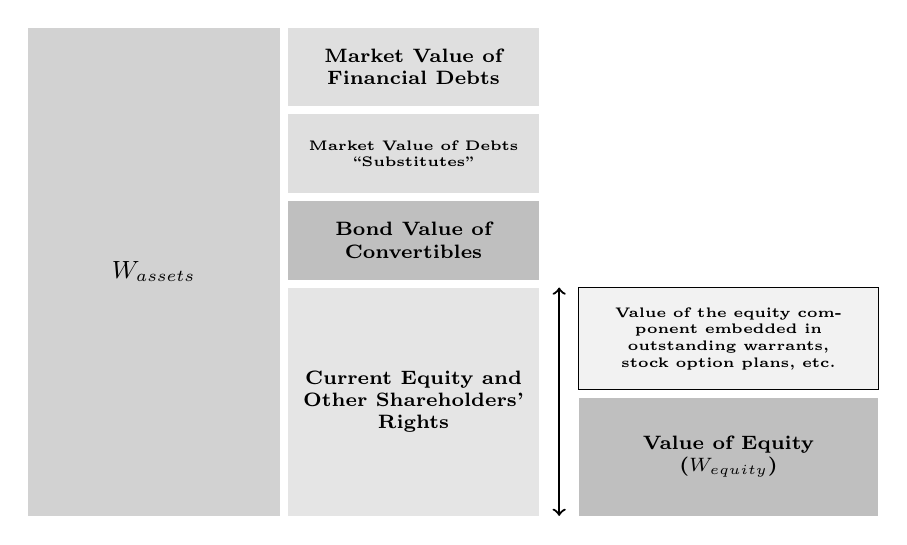
\begin{tikzpicture}[font=\small]
\fill[gray!35] (0,0) rectangle (3.2,6.2); \node[font=\small\bfseries] at (1.6,3.1) {$W_{\text{assets}}$};
\fill[gray!25] (3.3,5.2) rectangle (6.5,6.2); \node[align=center,font=\scriptsize\bfseries] at (4.9,5.7) {Market Value of\\Financial Debts};
\fill[gray!25] (3.3,4.1) rectangle (6.5,5.1); \node[align=center,font=\tiny\bfseries] at (4.9,4.6) {Market Value of Debts\\``Substitutes''};
\fill[gray!50] (3.3,3.0) rectangle (6.5,4.0); \node[align=center,font=\scriptsize\bfseries] at (4.9,3.5) {Bond Value of\\Convertibles};
\fill[gray!20] (3.3,0) rectangle (6.5,2.9); \node[align=center,font=\scriptsize\bfseries] at (4.9,1.45) {Current Equity and\\Other Shareholders'\\Rights};
\draw[<->,thick] (6.75,0) -- (6.75,2.9);
\fill[gray!10] (7.0,1.6) rectangle (10.8,2.9); \draw (7.0,1.6) rectangle (10.8,2.9); \node[align=center,font=\tiny\bfseries,text width=3.5cm] at (8.9,2.25) {Value of the equity component embedded in outstanding warrants, stock option plans, etc.};
\fill[gray!50] (7.0,0) rectangle (10.8,1.5); \node[align=center,font=\scriptsize\bfseries] at (8.9,0.75) {Value of Equity\\($W_{\text{equity}}$)};
\end{tikzpicture}
\end{center}

\begin{addbox}
A convertible bond = straight bond + conversion option. Its bond part is a debt claim; its option part is an equity-like claim. Warrants and employee stock options are also claims on equity, so to obtain the value of the existing shares you must subtract their value from total equity.
\end{addbox}

% =====================================================================
\section{Earnings and Cash Flows}

\subsection{Reorganization of the Balance Sheet: The Functional View}

To construct cash flows we use the \textbf{functional reorganization of the balance sheet}: aggregation of assets and liabilities \textbf{based on the business operations they belong to}.

\begin{center}
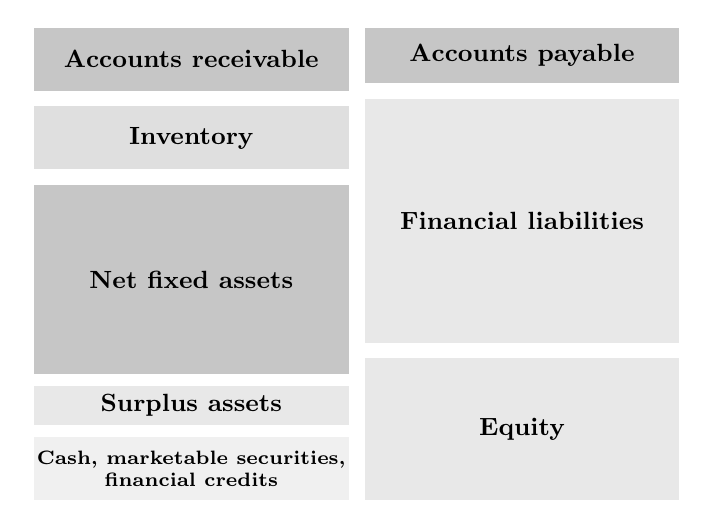
\begin{tikzpicture}[font=\small\bfseries]
\fill[gray!45] (0,5.2) rectangle (4,6.0); \node at (2,5.6) {Accounts receivable};
\fill[gray!25] (0,4.2) rectangle (4,5.0); \node at (2,4.6) {Inventory};
\fill[gray!45] (0,1.6) rectangle (4,4.0); \node at (2,2.8) {Net fixed assets};
\fill[gray!18] (0,0.95) rectangle (4,1.45); \node at (2,1.2) {Surplus assets};
\fill[gray!12] (0,0) rectangle (4,0.8); \node[font=\scriptsize\bfseries,align=center] at (2,0.4) {Cash, marketable securities,\\financial credits};
\fill[gray!45] (4.2,5.3) rectangle (8.2,6.0); \node at (6.2,5.65) {Accounts payable};
\fill[gray!18] (4.2,2.0) rectangle (8.2,5.1); \node at (6.2,3.55) {Financial liabilities};
\fill[gray!18] (4.2,0) rectangle (8.2,1.8); \node at (6.2,0.9) {Equity};
\end{tikzpicture}
\end{center}

\begin{keybox}[Principle]
Accounting classifies items for reporting; \textbf{valuation reorganizes them by economic function}.
\end{keybox}

\subsubsection*{Net working capital and net invested capital}

The categories related to the cycle of business operations are: $+$ Inventory, $+$ Accounts receivable, $-$ Accounts payable (for goods/services related to operations).

\begin{keybox}[Operating Net Working Capital]
The algebraic sum of these categories yields the \textbf{operating Net Working Capital (NWC)}:
\[
\text{NWC} = \text{Inventory} + \text{Accounts receivable} - \text{Accounts payable}
\]
\end{keybox}

The \textbf{net (operating) invested capital (NIC)} is composed of:
\begin{enumerate}
  \item \textbf{Net (operating) assets} (NA), i.e., operating assets net of D\&A and impairment losses. The size of the fixed assets relative to business volume depends on the \textbf{capital intensity index}, i.e., on the business-technical characteristics of the production process.
  \item \textbf{Working capital} (WC). For a given business volume, its size is directly related to the \textbf{length of the financial cycle} of the business operations (buy -- transform -- sell).
\end{enumerate}

\begin{center}
\begin{tikzpicture}[font=\small]
\fill[gray!60] (0,6.2) rectangle (3.5,6.8); \fill[gray!20] (0,5.9) rectangle (3.5,6.2);
\draw[decorate,decoration={brace,amplitude=4pt}] (-0.1,5.9) -- (-0.1,6.8) node[midway,left=5pt,align=right] {Accounts\\receivable};
\fill[gray!20] (0,4.0) rectangle (3.5,5.7); \node[font=\small\bfseries] at (1.75,4.85) {Inventories};
\fill[gray!50] (0,0) rectangle (3.5,3.8); \node[font=\small\bfseries] at (1.75,1.9) {Fixed assets};
\fill[gray!60] (3.8,6.2) rectangle (7.3,6.8); \node[font=\small\bfseries] at (5.55,6.5) {Accounts payable};
\draw[{Stealth}-{Stealth},thick] (4.3,6.1) -- (4.3,4.0) node[midway,right] {\textbf{WC}};
\draw[{Stealth}-{Stealth},thick] (4.3,3.8) -- (4.3,0) node[midway,right] {\textbf{NA}};
\draw[{Stealth}-{Stealth},thick] (6.6,6.1) -- (6.6,0) node[midway,right] {\textbf{NIC}};
\end{tikzpicture}
\end{center}

\begin{keybox}[Net invested capital]
\[
\text{NIC} = \text{NA} + \text{WC} = \text{Fixed assets} + \text{Inventories} + \text{Receivables} - \text{Payables}
\]
\end{keybox}

\subsubsection*{Benefits of the functional reorganization}
\begin{itemize}
  \item A \textbf{precise link between the balance-sheet values and their flows in the income statement}. This allows a rigorous analysis of profitability and simplifies the construction of economic and financial plans.
  \item A specific category of revenues and costs for \textbf{non-core activities} lets us value separately (i) the company's \textbf{core assets} and (ii) the \textbf{surplus assets}.
  \item To value the company as a \textbf{sum of parts (SOP)}, reconstruct the costs of each separate business area, normally \textbf{up to the EBIT level}.
\end{itemize}

\subsubsection*{How the assets are financed}

The net (operating and non-operating) assets are covered by (i) \textbf{financial liabilities} negotiated by the company (short and medium/long term) and (ii) \textbf{equity}.

\begin{center}
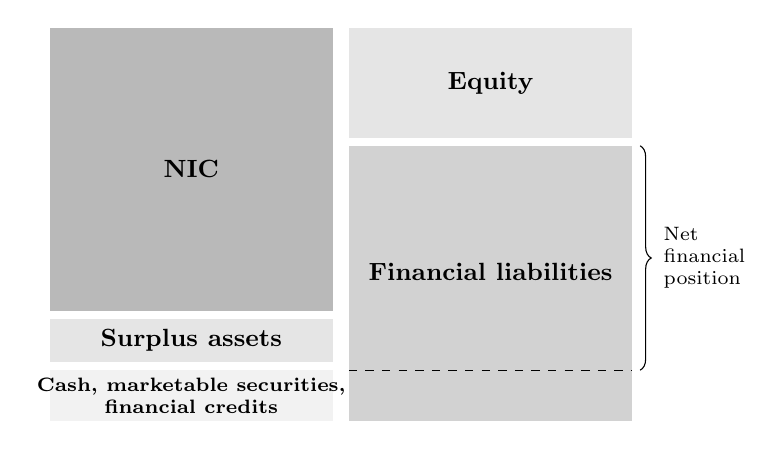
\begin{tikzpicture}[font=\small\bfseries]
\fill[gray!55] (0,1.4) rectangle (3.6,5.0); \node at (1.8,3.2) {NIC};
\fill[gray!20] (0,0.75) rectangle (3.6,1.3); \node at (1.8,1.03) {Surplus assets};
\fill[gray!10] (0,0) rectangle (3.6,0.65); \node[font=\scriptsize\bfseries,align=center] at (1.8,0.33) {Cash, marketable securities,\\financial credits};
\fill[gray!20] (3.8,3.6) rectangle (7.4,5.0); \node at (5.6,4.3) {Equity};
\fill[gray!35] (3.8,0) rectangle (7.4,3.5); \node at (5.6,1.9) {Financial liabilities};
\draw[dashed] (3.8,0.65) -- (7.4,0.65);
\draw[decorate,decoration={brace,amplitude=4pt}] (7.5,3.5) -- (7.5,0.65) node[midway,right=5pt,align=left,font=\scriptsize] {Net\\financial\\position};
\end{tikzpicture}
\end{center}

\begin{keybox}[Financial structure]
\[
\text{Net financial position} = \text{Financial liabilities} - \text{Cash \& cash equivalents}
\]
The proportion of the net financial position relative to equity determines the \textbf{financial structure} of the company.
\end{keybox}

\subsection{Reorganization of the Income Statement: ``At Added Value''}

\textbf{Why we care: FCFO starts from operating income, not net income.}

\begin{center}
\begin{tabular}{@{}l@{}}
\toprule
\textbf{\color{bocconi}1. Sales revenues}, or production value achieved during the fiscal year\\
\quad $-$ Consumption of raw materials and components acquired from third parties\\
\quad $-$ Costs of services acquired from outside (e.g., supplies, ads, etc.)\\
\quad $-$ Other external expenses (e.g., administration and control, organization, finance)\\
\midrule
\textbf{\color{bocconi}2. Added value}\\
\quad $-$ Labor costs\\
\midrule
\textbf{\color{bocconi}3. EBITDA} (Earnings Before Interest, Taxes, Depreciation, and Amortization)\\
\quad $-$ Depreciation \& Amortization and Provisions\\
\midrule
\textbf{\color{bocconi}4. Operating income or EBIT} (Earnings Before Interest and Taxes)\\
\quad $-$ Financial expenses ($+$ financial revenues) / $+$ Net result from non-core activities\\
\midrule
\textbf{\color{bocconi}5. Gross operating income from continuing operations}\\
\quad $-$ Extraordinary losses ($+$ extraordinary gains)\\
\midrule
\textbf{\color{bocconi}6. EBT} (Earnings Before Taxes)\\
\quad $-$ Tax expenses\\
\midrule
\textbf{\color{bocconi}7. Net income}\\
\bottomrule
\end{tabular}
\end{center}

\subsection[From Earnings to Cash Flows: Introduction]{From Earnings to Cash Flows: Introduction \layer{CORE}}

Our goal is to consider \textbf{all monetary inflows and outflows for all business areas}. Jointly, these flows determine the firm's financial dynamics in a certain period. The forces underlying a firm's financial dynamics include:
\begin{itemize}
  \item continuing business operations and related investment/divestment in net working capital;
  \item investment and divestment in fixed assets;
  \item underwriting and repayment of financing instruments (including issuance of equity capital);
  \item payment of interest/dividends to debt/equity holders;
  \item net flows from the purchase or disposal of surplus assets.
\end{itemize}
These forces are reorganized into: (1) \textbf{monetary flows of the operating area}; (2) \textbf{of the financing area}; (3) \textbf{of the non-core area}.

\subsection[Operating Area]{Operating Area \layer{CORE}}

The cash generated by current business operations is obtained by adding to the operating result all costs that do not generate monetary transactions (mainly D\&A in industrial companies): \textbf{this figure is EBITDA}.

\begin{itemize}
  \item \textbf{EBITDA is not free cash flow: working capital can absorb cash.}
  \item You cannot always use EBITDA to finance outflows unrelated to current activities. The cash actually available depends on the \textbf{change in NWC} in the period. A positive change in NWC mirrors an \textbf{employment of cash}, which absorbs part of EBITDA. Therefore:
\end{itemize}
\begin{keybox}
\[
\text{Monetary flow of current activities} = \text{EBITDA} \pm \Delta \text{WC}
\]
(an increase in WC is subtracted; a decrease is added)
\end{keybox}

\begin{addbox}
Example: EBITDA $=100$. Receivables grow by $30$ because sales grew and customers pay at 60 days. Those $30$ of revenue are already in EBITDA but have not yet been collected, so cash from current activities $=100-30=70$.
\end{addbox}

\subsection[Financing Area]{Financing Area \layer{PRO}}

The monetary flow from the financing area includes all movements relating to debt and equity capital:
\begin{center}
\begin{tabular}{@{}rl@{}}
$-$ & Passive interest payment\\
$-$ & Dividend distribution\\
$+$ & New debt negotiations\\
$-$ & Expiring debt repayment\\
$+$ & Equity increases\\
$-$ & Equity repayment\\
\midrule
$=$ & \textbf{Monetary flow from the financing area}
\end{tabular}
\end{center}
All these flows are calculated \textbf{net of fiscal adjustments for the company} (not for debt- or equity-holders), e.g., interest after the corporate tax shield.

\subsection[Non-Core Area]{Non-Core Area \layer{PRO}}

The flow from surplus (non-core) assets is easy to compute because few elements belong to this residual category. It has two components:
\begin{enumerate}
  \item the \textbf{income from non-core businesses};
  \item the difference between \textbf{new investments in} and \textbf{divestments of} non-core businesses.
\end{enumerate}
Again, \textbf{net of fiscal adjustments for the company}.

\subsection{TECH Layer: Reconciling the Statements}

\begin{keybox}[TECH layer]
The formulas are simple enough; the model is harder. \textbf{Every item must reconcile across the income statement, balance sheet, and cash-flow statement.}
\end{keybox}

\subsubsection*{Mechanics -- Part 1: Exhibit 3.4 (balance-sheet changes $\to$ cash-flow statement)}

\begin{figure}[H]
\centering
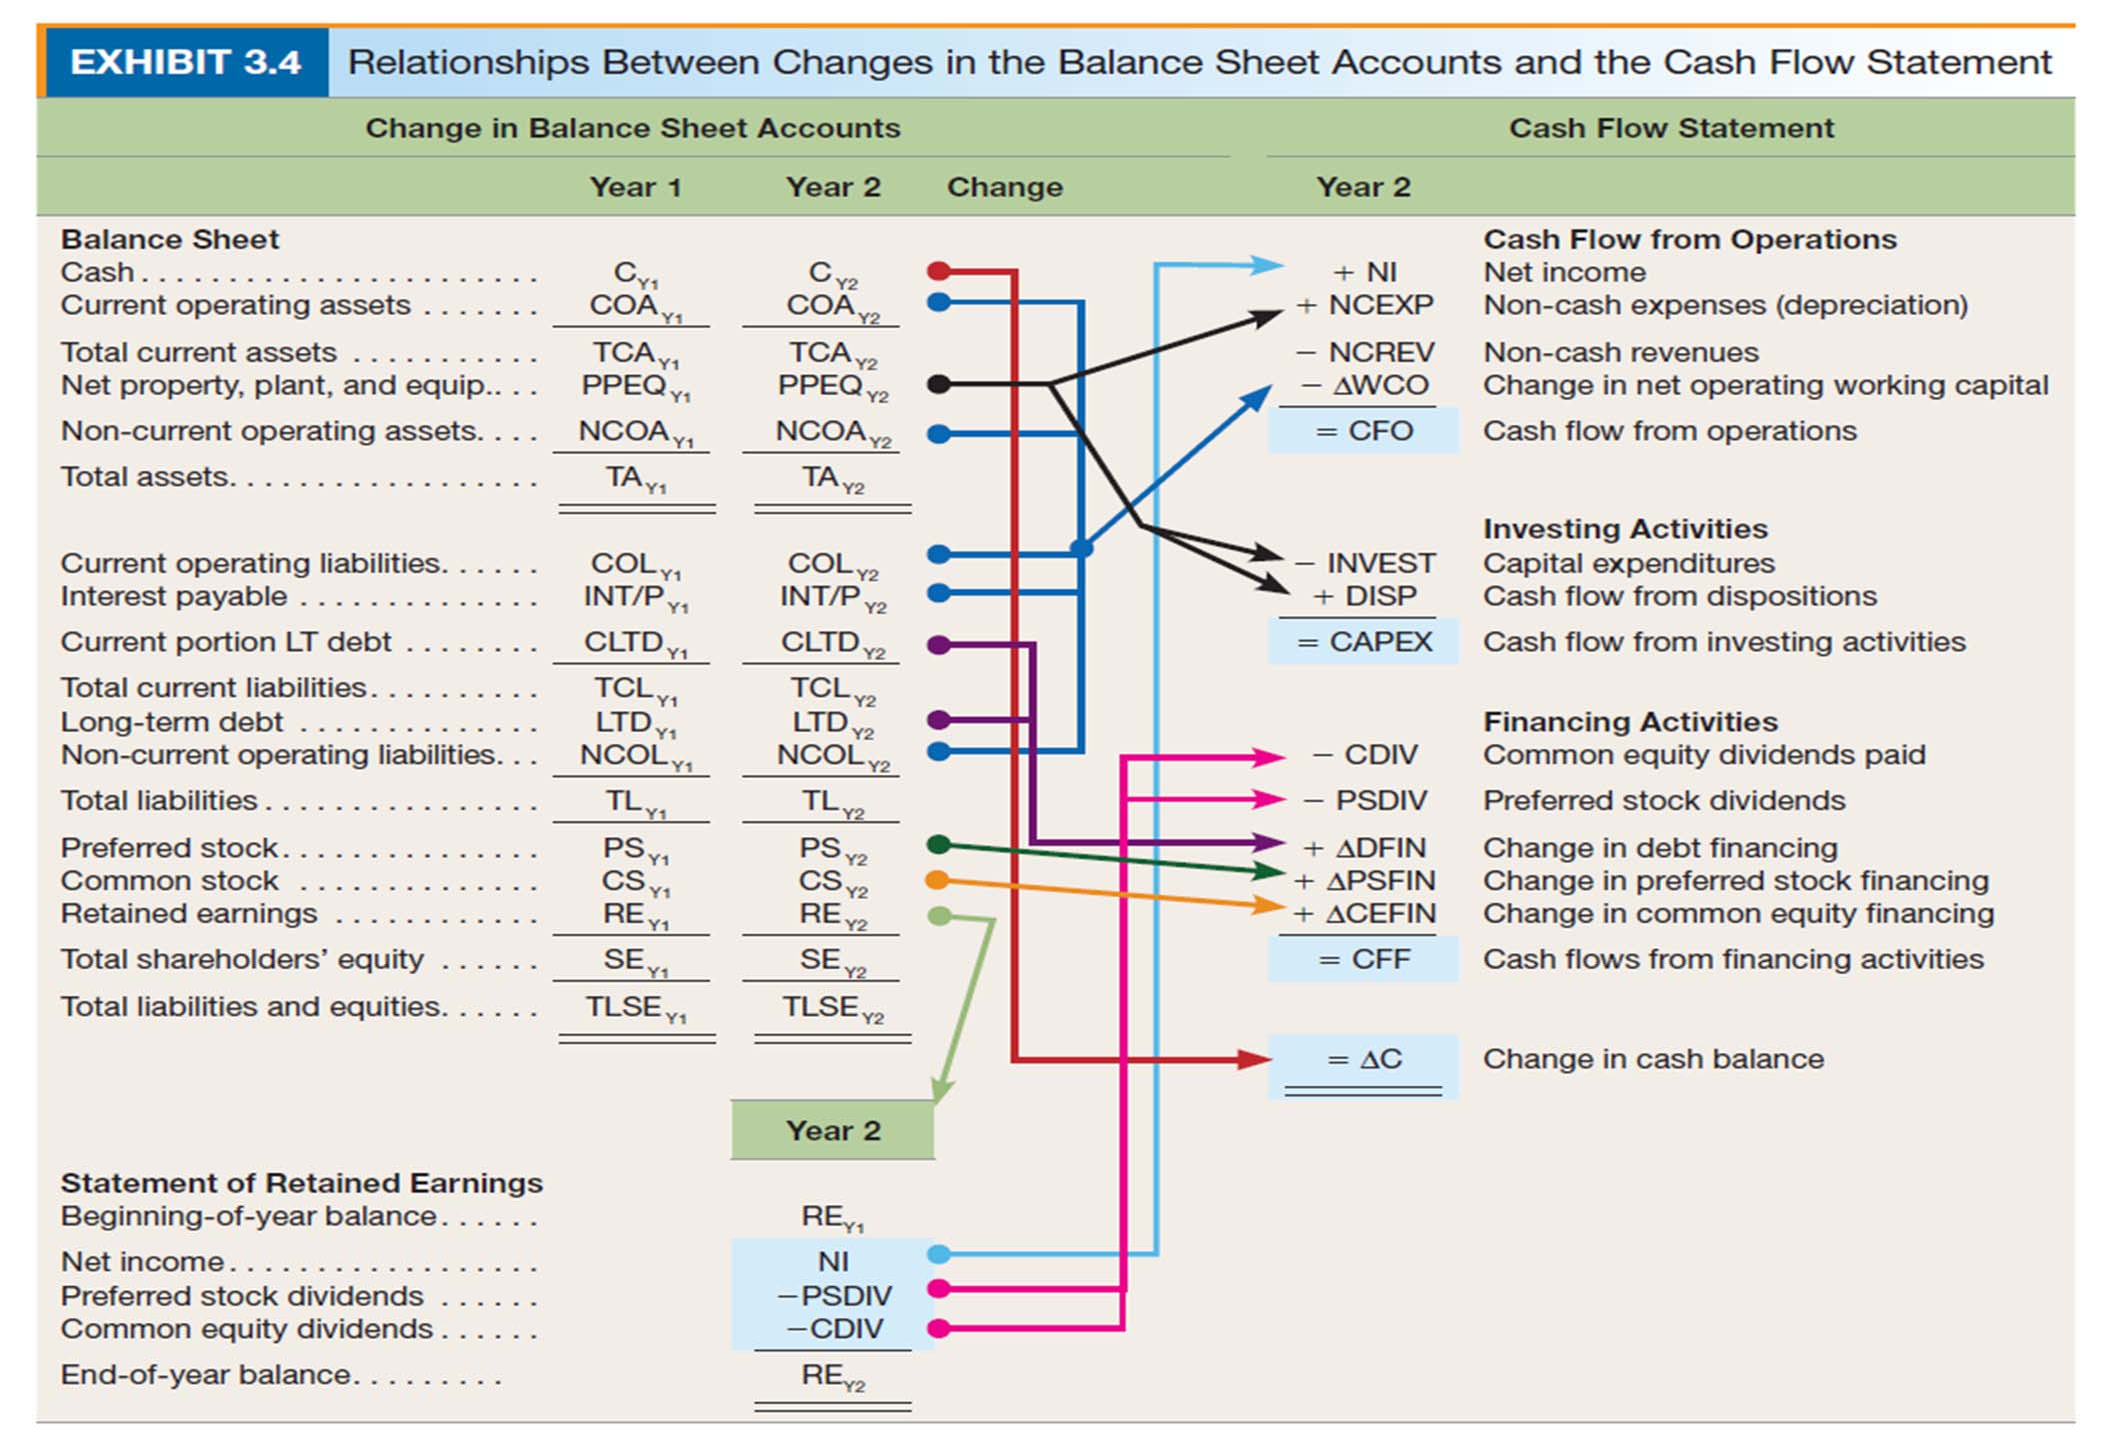
\includegraphics[width=\textwidth]{exhibit34.png}
\caption{Holthausen--Zmijewski, Exhibit 3.4: relationships between changes in the balance-sheet accounts and the cash-flow statement (slide screenshot).}
\end{figure}

Reading the arrows of Exhibit 3.4:
\begin{center}
\small
\begin{tabularx}{\textwidth}{@{}Xl@{}}
\toprule
\textbf{Change in balance-sheet account} & \textbf{Line of the cash-flow statement}\\
\midrule
$\Delta$ Cash ($C$) & $=\Delta C$ (change in cash balance)\\
$\Delta$ Current operating assets (COA), $\Delta$ non-current operating assets (NCOA), $\Delta$ current operating liabilities (COL), $\Delta$ interest payable (INT/P), $\Delta$ non-current operating liabilities (NCOL) & $-\Delta$WCO (in CFO)\\
$\Delta$ Net PP\&E (PPEQ) & $+$NCEXP (CFO); $-$INVEST, $+$DISP (investing)\\
$\Delta$ Current portion of LT debt (CLTD), $\Delta$ long-term debt (LTD) & $+\Delta$DFIN\\
$\Delta$ Preferred stock (PS) & $+\Delta$PSFIN\\
$\Delta$ Common stock (CS) & $+\Delta$CEFIN\\
$\Delta$ Retained earnings: $RE_{Y1}+NI-PSDIV-CDIV=RE_{Y2}$ & $+$NI (CFO); $-$PSDIV, $-$CDIV (financing)\\
\bottomrule
\end{tabularx}
\end{center}

\begin{keybox}[Cash-flow statement]
\begin{align*}
\text{CFO} &= \text{NI} + \text{NCEXP} - \text{NCREV} - \Delta\text{WCO}\\
\text{Cash flow from investing (CAPEX)} &= -\text{INVEST} + \text{DISP}\\
\text{CFF} &= -\text{CDIV} - \text{PSDIV} + \Delta\text{DFIN} + \Delta\text{PSFIN} + \Delta\text{CEFIN}\\
\Delta \text{C} &= \text{CFO} + \text{Investing} + \text{CFF}
\end{align*}
\end{keybox}

\subsubsection*{Mechanics -- Part 2: Exhibit 3.8 (cash-flow statement $\to$ free-cash-flow schedule)}

\begin{figure}[H]
\centering
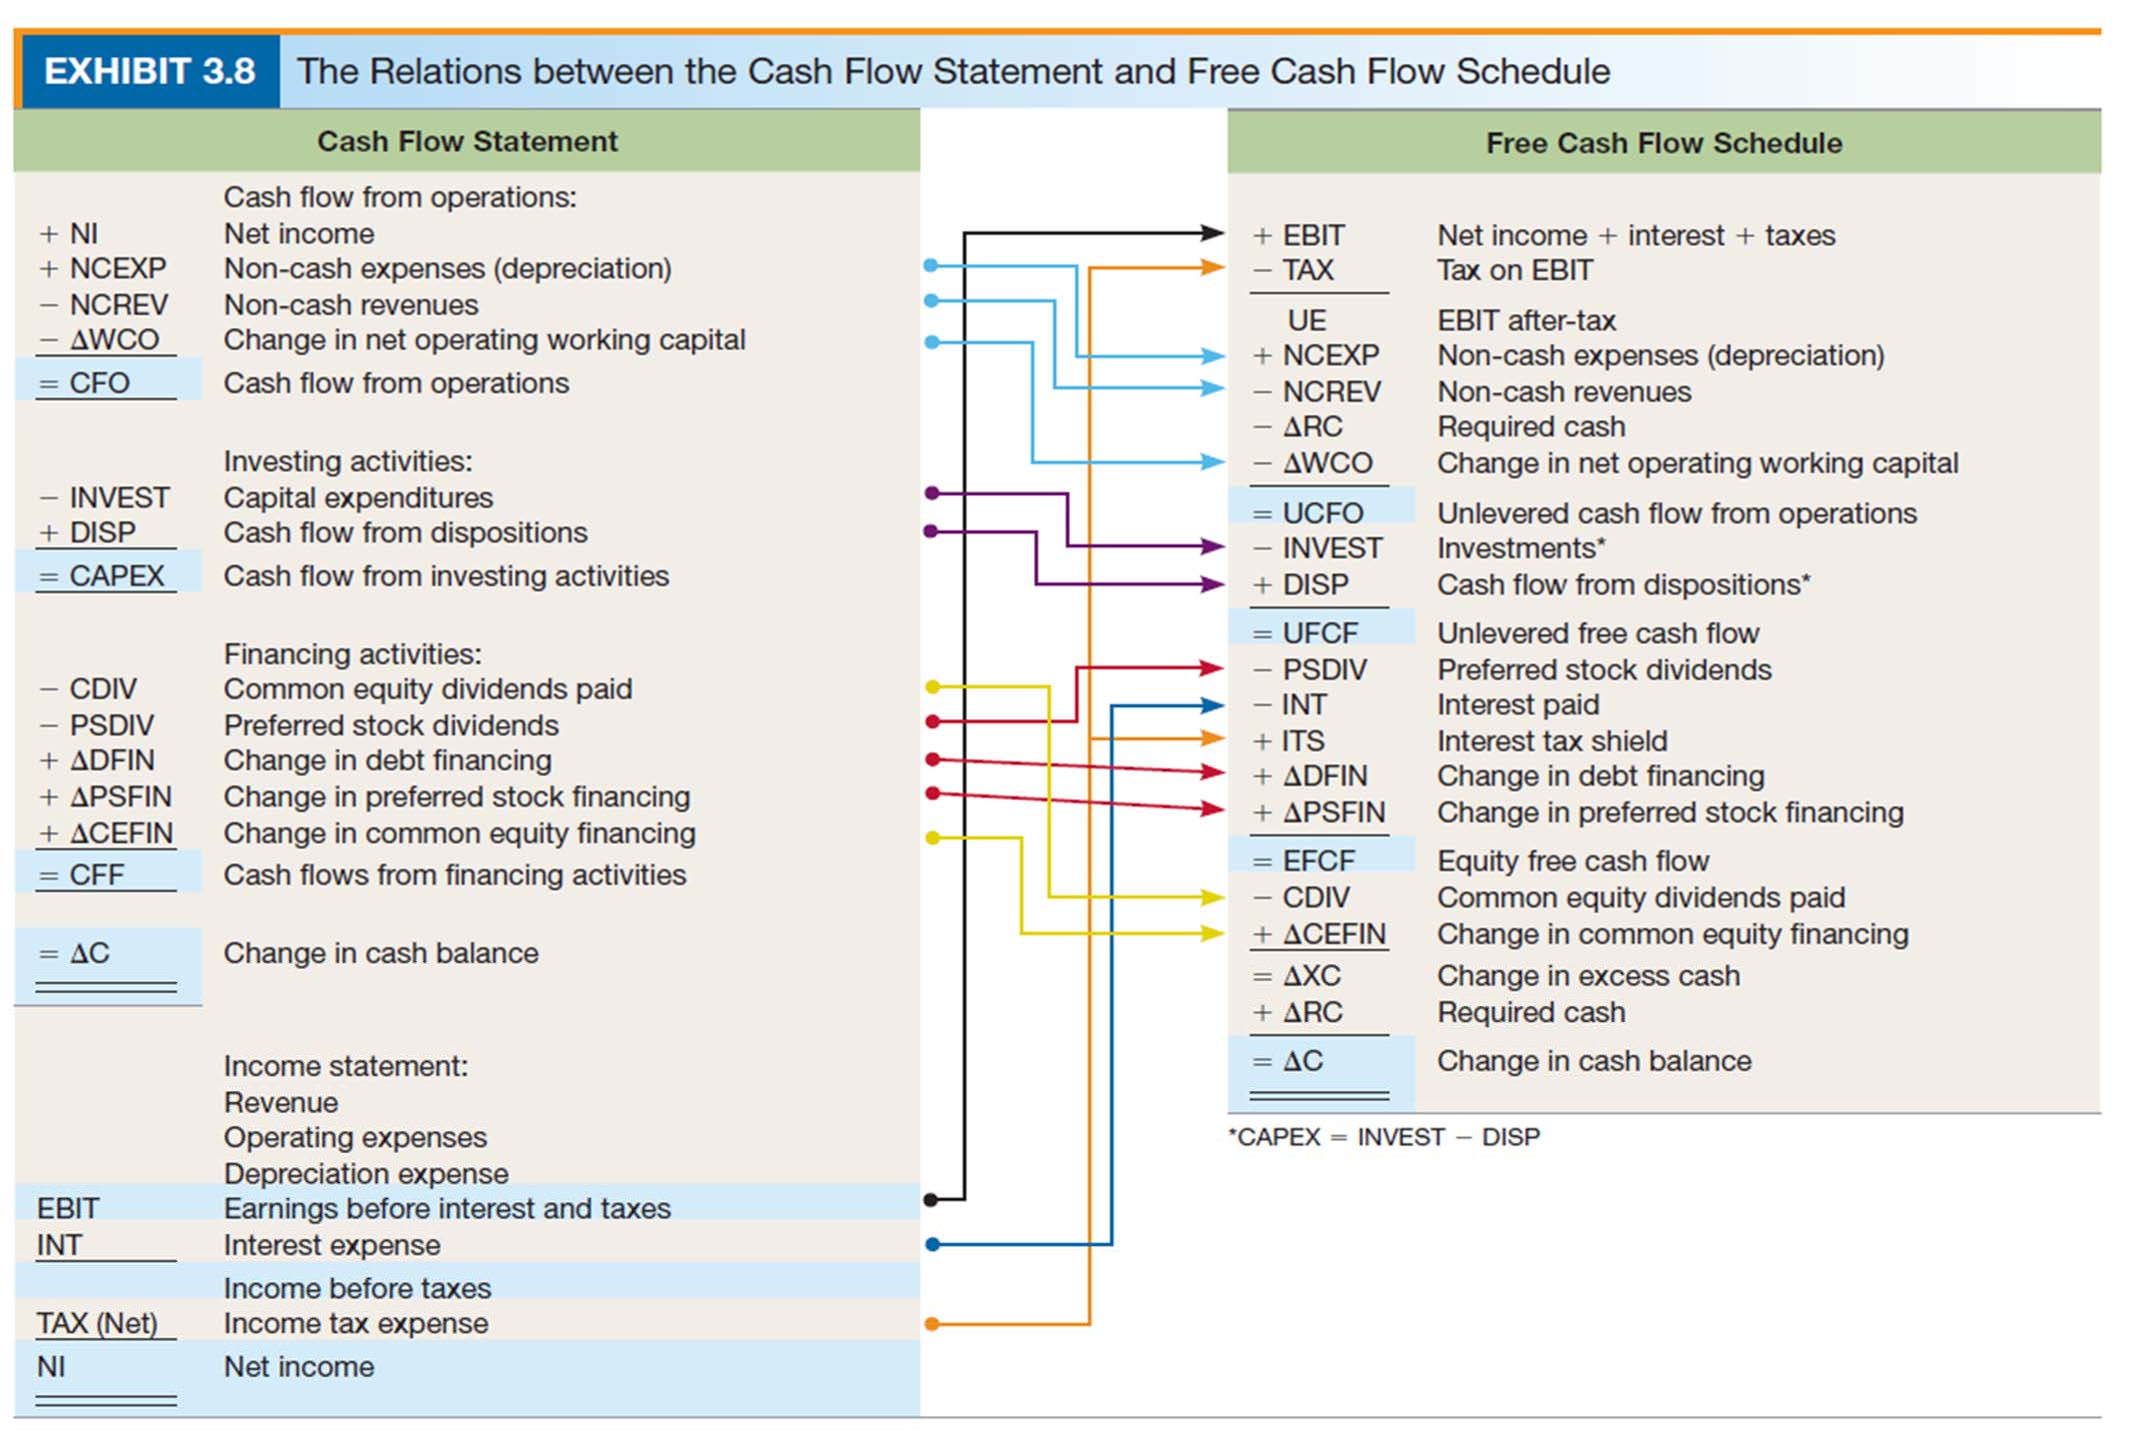
\includegraphics[width=\textwidth]{exhibit38.png}
\caption{Holthausen--Zmijewski, Exhibit 3.8: relations between the cash-flow statement and the free-cash-flow schedule (slide screenshot).}
\end{figure}

\begin{center}
\small
\begin{tabular}{@{}rll@{}}
\toprule
& \textbf{Line} & \textbf{Meaning}\\
\midrule
$+$ & EBIT & Net income + interest + taxes\\
$-$ & TAX & Tax on EBIT\\
\cmidrule{2-3}
& UE & EBIT after tax\\
$+$ & NCEXP & Non-cash expenses (depreciation)\\
$-$ & NCREV & Non-cash revenues\\
$-$ & $\Delta$RC & Required cash\\
$-$ & $\Delta$WCO & Change in net operating working capital\\
\cmidrule{2-3}
$=$ & \textbf{UCFO} & Unlevered cash flow from operations\\
$-$ & INVEST & Investments$^*$\\
$+$ & DISP & Cash flow from dispositions$^*$\\
\cmidrule{2-3}
$=$ & \textbf{UFCF} & \textbf{Unlevered free cash flow ($=$ FCFO)}\\
$-$ & PSDIV & Preferred stock dividends\\
$-$ & INT & Interest paid\\
$+$ & ITS & Interest tax shield\\
$+$ & $\Delta$DFIN & Change in debt financing\\
$+$ & $\Delta$PSFIN & Change in preferred stock financing\\
\cmidrule{2-3}
$=$ & \textbf{EFCF} & \textbf{Equity free cash flow ($=$ FCFE)}\\
$-$ & CDIV & Common equity dividends paid\\
$+$ & $\Delta$CEFIN & Change in common equity financing\\
\cmidrule{2-3}
$=$ & $\Delta$XC & Change in excess cash\\
$+$ & $\Delta$RC & Required cash\\
\cmidrule{2-3}
$=$ & $\Delta$C & Change in cash balance\\
\bottomrule
\multicolumn{3}{@{}l}{\footnotesize $^*$CAPEX $=$ INVEST $-$ DISP}
\end{tabular}
\end{center}

\begin{addbox}[What Exhibit 3.8 teaches]
\begin{enumerate}[leftmargin=*]
  \item The free-cash-flow schedule ends at the \textbf{same $\Delta C$} as the cash-flow statement, so the two reconcile.
  \item \textbf{Required cash} (the cash needed to run the business) is an \textbf{operating} investment, subtracted in UCFO like working capital. \textbf{Excess cash} is what is left after paying shareholders.
  \item \textbf{Tax on EBIT $\neq$ income-tax expense}: TAX on EBIT $=$ tax expense $+$ interest tax shield, with ITS $=t\times$INT. The ITS is given back to equity holders in EFCF.
  \item Dividends are \textbf{not} in FCFE; they are a \textbf{use} of FCFE: FCFE $-$ dividends $+$ new equity $=$ change in excess cash.
\end{enumerate}
\end{addbox}

\subsection{Two Cash-Flow Definitions to Remember}

\begin{keybox}[The two definitions -- memorize]
\begin{align*}
\text{FCFO} &= \text{EBIT}\times(1-\text{tax rate}) + \text{non-cash charges} - \text{CapEx} - \text{increase in non-cash WC}\\[4pt]
\text{FCFE} &= \text{net income} + \text{non-cash charges} - \text{CapEx} - \text{increase in non-cash WC}\\
&\quad + \text{net debt issued}
\end{align*}
\end{keybox}

\subsection{Cash-Flow Definitions in Full}

\begin{center}
\small\begin{tabular}{@{}rl@{\hspace{0.8cm}}rl@{}}
\multicolumn{2}{@{}l}{\textbf{1. FCFE -- equity-side valuation}} & \multicolumn{2}{l}{\textbf{2. FCFO -- asset-side valuation}}\\[3pt]
$+$ & Net income -- adjusted & $+$ & FCFE\\
$+/-$ & Non-cash expenditure (other than D\&A) & $+$ & Interest expense $\times(1-$tax rate$)$\\
& \quad / non-cash revenues & $+$ & (Principal debt repayments\\
$-$ & Net CapEx ($=$ CapEx $-$ D\&A) && \quad $-$ new debt issues)\\
\cmidrule{3-4}
$-$ & Changes in non-cash working capital & $=$ & \textbf{FCFO}\\[6pt]
$-$ & (Principal debt repayments & $+$ & Operating income (EBIT) -- adjusted\\
& \quad $-$ new debt issues) & $+/-$ & Non-cash expenditure (other than D\&A)\\
\cmidrule{1-2}
$=$ & \textbf{FCFE} && \quad / non-cash revenues\\
&& $-$ & Taxes on EBIT\\
&& $-$ & Reinvestment needs (net CapEx and WC)\\
\cmidrule{3-4}
&& $=$ & \textbf{FCFO}
\end{tabular}
\end{center}
\slidefig{[Ignoring preferred dividends. If preferred stock exists, preferred dividends also need to be netted out.]}

\begin{keybox}[FCFE $\leftrightarrow$ FCFO]
\[
\text{FCFE} = \text{FCFO} - \text{Interest}\times(1-t) + (\text{New debt issues} - \text{Principal repayments})
\]
\end{keybox}

\begin{addbox}[Proof that the two routes agree]
$NI=(\text{EBIT}-\text{Int})(1-t)=\text{EBIT}(1-t)-\text{Int}(1-t)$. Substituting into FCFE:
\[
\text{FCFE}=\underbrace{\text{EBIT}(1-t)+\text{D\&A}-\text{CapEx}-\Delta\text{WC}}_{\text{FCFO}}-\text{Int}(1-t)+\text{Net borrowing}.
\]
\end{addbox}

\subsection[Discussion Question]{Discussion Question \layer{PRACTICE}}

\begin{exbox}[Discussion Question -- data]
\begin{center}
\begin{tabular}{@{}lr@{}}
EBIT & \$400\\
Interest expensed and paid & \$100\\
Income tax rate on all income & 40\%\\
Net income & \$180\\
Depreciation & \$200\\
Capital expenditures & \$540\\
Increase in required non-cash working capital & \$80\\
Increase in required cash & \$20\\
Increase in debt financing & \$400\\
Paid-in common dividends & \$90\\
Change in cash balance on balance sheet & \$70\\
Cash flow from operations & \$300\\
\end{tabular}
\end{center}
(i) Prepare the cash-flow statement forecast; (ii) prepare the FCFO forecast; (iii) prepare the FCFE forecast.
\end{exbox}

\begin{exbox}[Solution -- \checkmark\ confirmed by the official class solution (CF-BVal\_02\_Bocconi\_2023\_SOL.xlsx, ``The Example Co'')]
\textbf{Check net income:} EBT $=400-100=300$; taxes $=300\times40\%=120$; NI $=300-120=180$ \checkmark

\medskip
\begin{minipage}[t]{0.47\textwidth}
\textbf{(i) Cash-flow statement}\\[3pt]
\begin{tabular}{@{}lr@{}}
Net income & 180\\
+ Depreciation & 200\\
$-$ Increase in non-cash WC & (80)\\
\midrule
\textbf{= CFO} & \textbf{300} \checkmark\\[3pt]
$-$ Capital expenditures & (540)\\
\midrule
\textbf{= Cash flow from investing} & \textbf{(540)}\\[3pt]
+ Increase in debt & 400\\
$-$ Common dividends & (90)\\
\midrule
\textbf{= CFF} & \textbf{310}\\[3pt]
\textbf{$\Delta$ Cash} $=300-540+310$ & \textbf{70} \checkmark
\end{tabular}
\end{minipage}\hfill
\begin{minipage}[t]{0.47\textwidth}
\textbf{(ii) FCFO}\\[3pt]
\begin{tabular}{@{}lr@{}}
EBIT & 400\\
$-$ Tax on EBIT ($400\times40\%$) & (160)\\
\midrule
= EBIT$(1-t)$ & 240\\
+ Depreciation & 200\\
$-$ Increase in required cash & (20)\\
$-$ Increase in non-cash WC & (80)\\
\midrule
= UCFO & 340\\
$-$ Capital expenditures & (540)\\
\midrule
\textbf{= FCFO} & \textbf{(200)}
\end{tabular}
\end{minipage}

\medskip
\textbf{(iii) FCFE}\\[3pt]
\begin{tabular}{@{}lr@{}}
FCFO & (200)\\
$-$ Interest paid & (100)\\
+ Interest tax shield ($100\times40\%$) & 40\\
+ Net debt issued & 400\\
\midrule
\textbf{= FCFE} & \textbf{140}
\end{tabular}

\medskip
Check from net income: FCFE $=180+200-540-80-20+400=\mathbf{140}$ \checkmark

\textbf{Reconciliation:} FCFE $140-$ dividends $90=$ change in excess cash $50$; $+$ increase in required cash $20=$ \textbf{change in cash $70$} \checkmark\ (matches the balance sheet).

\textbf{Notes.} Tax on EBIT (160) $\neq$ taxes actually paid (120); the difference (40) is the interest tax shield. If required cash were ignored, FCFO would be $-180$. The lecture stresses that ``required cash is not excess cash'', so required cash is an operating need and FCFO $=-200$ (the official solution confirms $-200$).
\end{exbox}

\begin{exbox}[Official solution, third schedule: from CFO to FCFO]
The class solution also derives FCFO starting from the cash-flow-statement CFO, undoing the financing items that CFO contains:
\begin{center}
\begin{tabular}{@{}llr@{}}
\toprule
Cash flow from operations & $+$ CFO & 300\\
$+$ Interest paid in cash & $+$ CINT & 100\\
$-$ Interest tax shield ($40\%\times100$) & $-$ ITS & (40)\\
$-$ Change in required cash & $-\Delta$RC & (20)\\
\midrule
Unlevered cash flow from operations & $=$ UCFO & 340\\
$-$ Capital expenditures & $-$ CAPEX & (540)\\
\midrule
\textbf{Unlevered free cash flow} & $=$ \textbf{FCF} & \textbf{(200)}\\
\bottomrule
\end{tabular}
\end{center}
Logic: CFO starts from net income, so it is \emph{after} interest net of its tax shield ($100\times(1-0.4)=60$). Adding back interest (100) and removing the tax shield (40) gives back exactly those 60, i.e.\ the unlevered figure. Required cash, which CFO ignores, is an operating investment. The official FCF schedule also shows the line \emph{Cash flow before changes in financing} (CFBFIN) $=$ FCF $-$ interest $+$ ITS $-$ preferred dividends $=-200-100+40=-260$, then $+400$ of new debt $=$ EFCF 140.
\end{exbox}

\textbf{What these Discussion Questions test} (slide):
\begin{enumerate}
  \item \textbf{CFO is not FCFO} (300 vs $-200$: CFO is after interest and before CapEx).
  \item \textbf{FCFO excludes (debt) financing} (the 400 of new debt does not enter FCFO).
  \item \textbf{FCFE includes net debt issuance} ($+400$).
  \item \textbf{Dividends are a use of FCFE, not part of FCFO} (the 90 appears only after FCFE).
  \item \textbf{Required cash is not excess cash} (the 20 is an operating investment).
\end{enumerate}

\begin{addbox}
FCFO is negative here because the firm is in an investment phase (CapEx 540 $\gg$ depreciation 200). A negative FCFO is not ``bad'' in itself, since a growing firm reinvests. Here it was financed with new debt, which makes FCFE positive.
\end{addbox}

\subsection{Cash-Flow Definitions: Interpretation}

\begin{itemize}
  \item These concepts apply to \textbf{projections} used in valuation techniques.
  \item \textbf{FCFO}, also known as \textbf{Free Cash Flow to Firm (FCFF)}: the cash flows generated by the operating business. In FCFO the taxes measure the \textbf{theoretical fiscal outflow on the operating result in a scenario of no debt}.
  \item \textbf{FCFE}: the net cash flows available to shareholders. Its value depends not only on interest and income taxes but also on the \textbf{change in the net financial position}. Therefore the projections for the valuation must include a \textbf{target for the firm's financial structure}, because FCFE depends on future financing choices involving debt.
\end{itemize}

% =====================================================================
\subsection{From Reported to Actual Earnings}

\begin{center}
\begin{tikzpicture}[font=\small,
  bx/.style={draw,rounded corners=3pt,align=center,inner sep=4pt,fill=white,drop shadow},
  ln/.style={-{Stealth},thick}]
\node[bx] (h) at (0,3) {Firm's\\history};
\node[bx] (c) at (2.1,3) {Comparable\\Firms};
\node[bx,align=left] (ol) at (4.9,3) {\textbf{\emph{Operating leases}}\\- Convert into debt\\- Adjust operating\\\ \ income};
\node[bx,align=left] (rd) at (8.5,3) {\textbf{\emph{R\&D Expenses}}\\- Convert into asset\\- Adjust operating\\\ \ income};
\node[bx] (n) at (1.05,0.9) {\textbf{Normalize}\\\textbf{Earnings}};
\node[bx,align=left] (cl) at (6.7,0.9) {\textbf{Cleanse} operating items of\\- Financial Expenses\\- Capital Expenses\\- Non-recurring expense};
\node[draw=navy,thick,ellipse,fill=boxblue,font=\normalsize\bfseries] (m) at (4,-0.9) {Measuring Earnings};
\node[bx,draw=teal,align=left] (u) at (7.6,-2.2) {\textbf{Update}\\- Trailing Earnings\\- Unofficial numbers};
\draw[thick] (h.south) |- (1.05,2.1) -| (c.south); \draw[ln] (1.05,2.1) -- (n.north);
\draw[thick] (ol.south) |- (6.7,1.95) -| (rd.south); \draw[ln] (6.7,1.95) -- (cl.north);
\draw[thick] (n.south) |- (4,-0.15) ; \draw[thick] (cl.south) |- (4,-0.15); \draw[ln] (4,-0.15) -- (m.north);
\draw[ln] (u.west) -| (4,-1.35);
\end{tikzpicture}
\end{center}

\subsubsection*{Adjusting accounting earnings}
\begin{enumerate}
  \item \textbf{Make sure no financial expenses are mixed in with operating expenses.}
  \begin{itemize}
    \item \textbf{Financial expense}: any \textbf{tax-deductible commitment that you have to meet no matter what your operating results}. Failure to meet it leads to loss of control of the business.
    \item Example -- \textbf{operating leases}: accounting convention may treat them as operating expenses, but they are really financial expenses and must be reclassified. \textbf{This has no effect on equity earnings but does change the operating earnings.}
  \end{itemize}
  \item \textbf{Make sure no capital expenses (CAPEX) are mixed in with operating expenses (OPEX).}
  \begin{itemize}
    \item \textbf{Capital expense}: any expense that is expected to generate \textbf{benefits over multiple periods}.
    \item Example -- \textbf{R\&D}: since R\&D is a capital expenditure (rather than an operating expense), the operating income has to be adjusted to reflect its treatment.
  \end{itemize}
\end{enumerate}

\subsection{Operating Leases}

\begin{center}
\begin{tikzpicture}
\begin{axis}[ybar,width=11cm,height=5.5cm,bar width=24pt,ymin=0,ymax=60,
  ylabel={\% of operating income},yticklabel={\pgfmathprintnumber{\tick}\%},
  symbolic x coords={Market,Apparel Stores,Furniture Stores,Restaurants},xtick=data,
  xticklabel style={align=center,text width=1.8cm},xticklabels={Market,Apparel\\Stores,Furniture\\Stores,Restaurants},
  title={\small Operating lease expenses as \% of operating income},
  nodes near coords={\pgfmathprintnumber{\pgfplotspointmeta}\%},nodes near coords style={font=\scriptsize},
  ymajorgrids,tick label style={font=\small},enlarge x limits=0.18]
\addplot[fill=navy!45,draw=navy] coordinates {(Market,12.5) (Apparel Stores,43.5) (Furniture Stores,49.5) (Restaurants,26.5)};
\end{axis}
\end{tikzpicture}
\slidefig{Values read from the slide's bar chart (approximate). Leases matter most for retailers and restaurants.}
\end{center}

\begin{itemize}
  \item Operating lease expenses may be treated as operating expenses in computing operating income.
  \item More appropriately, they should be treated as \textbf{financing expenses}, with the following adjustments to earnings and capital:
  \begin{itemize}
    \item \textbf{Debt value of operating leases = PV of operating lease commitments at the pre-tax cost of debt.}
    \item When you convert operating leases into debt, you also create an \textbf{asset of the same value} to counter it.
  \end{itemize}
\end{itemize}

\begin{keybox}[Adjusted operating earnings]
\begin{align*}
\text{Adj.\ operating earnings} &= \text{Operating earnings} + \text{Op.\ lease expense}\\
&\quad - \text{Depreciation on leased asset}\\
\intertext{As an approximation:}
\text{Adj.\ operating earnings} &\approx \text{Operating earnings} + \text{Pre-tax cost of debt}\times\text{PV of op.\ leases}
\end{align*}
\end{keybox}

\begin{addbox}
A lease payment is economically interest + repayment of a loan. Adding back the whole payment and subtracting only the depreciation of the leased asset removes the financing cost (the implicit interest) from operating expenses. The approximation adds back only the imputed interest ($k_d\times$ lease debt), on the assumption that depreciation $\approx$ the principal part of the payment.
\end{addbox}

\begin{exbox}[Worked example: The GAP]
GAP has EBIT of \$1,012m and debt of \$1.97bn; pre-tax cost of debt $6\%$. Operating lease payments this year \$978m. Commitments:
\begin{center}
\begin{tabular}{@{}crcr@{}}
\toprule
\textbf{Year} & \textbf{Commitment (\$m)} & \textbf{$1/1.06^t$} & \textbf{PV at 6\%}\\
\midrule
1 & 899.00 & 0.94340 & 848.11\\
2 & 846.00 & 0.89000 & 752.94\\
3 & 738.00 & 0.83962 & 619.64\\
4 & 598.00 & 0.79209 & 473.67\\
5 & 477.00 & 0.74726 & 356.44\\
6 & 982.50 & 0.70496 & 692.62\\
7 & 982.50 & 0.66506 & 653.42\\
\midrule
6 \& 7 & 982.50 each year & & \textbf{1,346.04}\\
\multicolumn{3}{@{}r}{\textbf{Debt value of leases} (also value of leased asset) $=$} & \textbf{4,396.85}\\
\bottomrule
\end{tabular}
\end{center}
\textcolor{keyred}{\textbf{Slide typo:}} the slide shows \$1,356.04 for years 6--7; the correct value is \textbf{\$1,346.04}, the only figure consistent with the slide's total of \$4,396.85.

\begin{align*}
\text{Adjusted debt outstanding} &= 1{,}970 + 4{,}397 = \mathbf{\$6{,}367m}\\
\text{Adjusted EBIT} &= \text{Reported EBIT} + \text{OL exp.\ this year} - \text{Depreciation}\\
&= 1{,}012 + 978 - \tfrac{4{,}397}{7} = 1{,}012+978-628 = \mathbf{\$1{,}362m}\\[-2pt] &\qquad\text{(7-year useful life of the leased assets, straight line)}\\
\text{Approximate EBIT} &= 1{,}012 + 4{,}397\times6\% = 1{,}012+264 = \mathbf{\$1{,}276m}
\end{align*}
\added Commitments beyond year 5 are often disclosed as a lump sum (here $1{,}965=2\times982.5$) and spread evenly over the remaining years.
\end{exbox}

\begin{exbox}[GAP: conventional accounting vs operating leases treated as debt]
\small
\begin{tabularx}{\linewidth}{@{}>{\bfseries}p{2.1cm}XX@{}}
\toprule
& \textbf{\color{keyred}Conventional accounting} & \textbf{\color{keyred}Operating leases treated as debt}\\
\midrule
Income statement & EBIT before leases $=1{,}990$\newline Op.\ leases $=978$\newline EBIT $=1{,}012\ (=1{,}990-978)$ & EBIT before leases $=1{,}990$\newline $-$ Depreciation leased assets $=628$\newline Adjusted EBIT $=1{,}362\ (=1{,}990-628)$\newline \emph{Interest expense rises to reflect the conversion of operating leases into debt.}\\
\midrule
Balance sheet & Off balance sheet (shown neither as debt nor as an asset). Only the conventional debt of \$1,970m is on the balance sheet. & Asset: OL asset 4,397; Liability: OL debt 4,397\newline Total debt $=4{,}397+1{,}970=\$6{,}367$m\\
\midrule
Cost of capital & $8.20\%\cdot\frac{7{,}350}{9{,}320}+4\%\cdot\frac{1{,}970}{9{,}320}=\mathbf{7.31\%}$ & $8.20\%\cdot\frac{7{,}350}{13{,}717}+4\%\cdot\frac{6{,}367}{13{,}717}=\mathbf{6.25\%}$\\
& \multicolumn{2}{l}{\emph{Cost of equity 8.20\%; after-tax cost of debt 4\%; market value of equity 7,350.}}\\
\midrule
ROIC & $\frac{1{,}012(1-0.35)}{3{,}130+1{,}970}=\frac{657.8}{5{,}100}=\mathbf{12.90\%}$ & $\frac{1{,}362(1-0.35)}{3{,}130+6{,}367}=\frac{885.3}{9{,}497}=\mathbf{9.30\%}$\\
& \multicolumn{2}{l}{\emph{Book value of equity 3,130; tax rate 35\%.}}\\
\bottomrule
\end{tabularx}
\smallskip

\footnotesize $9{,}320=7{,}350+1{,}970$; $13{,}717=7{,}350+6{,}367$. Unrounded, the adjusted ROIC is 9.32\%; the slide shows 9.30\%.
\end{exbox}

\begin{addbox}[Summary of the lease effects]
Capitalizing leases: \textbf{EBIT $\uparrow$, debt $\uparrow$, WACC $\downarrow$} (more weight on cheaper debt), \textbf{invested capital $\uparrow\Rightarrow$ ROIC $\downarrow$}. \textbf{Net income/equity earnings are unaffected} (the slide says so explicitly), and equity value is essentially unchanged: EV is higher, but more debt is subtracted.
\end{addbox}

\subsubsection*{IFRS 16}
\begin{itemize}
  \item In January 2016, \textbf{IFRS 16} was issued, superseding \textbf{IAS 17}.
  \item IFRS 16 applies to reporting periods beginning on or after \textbf{January 1st, 2019}.
  \item Under IFRS 16 \textbf{all leases have to be capitalized} (shown on the balance sheet of the lessee).
\end{itemize}

\begin{center}
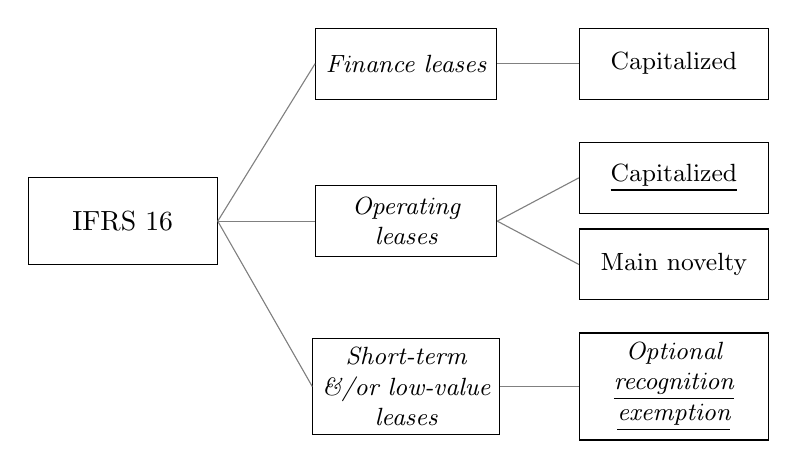
\begin{tikzpicture}[font=\small,
  r/.style={draw,minimum width=2.4cm,minimum height=0.9cm,align=center},
  m/.style={draw,minimum width=2.3cm,minimum height=0.9cm,align=center,font=\small\itshape}]
\node[r,minimum height=1.1cm,font=\normalsize] (i) at (0,0) {IFRS 16};
\node[m] (f) at (3.6,2.0) {Finance leases};
\node[m] (o) at (3.6,0) {Operating\\leases};
\node[m] (s) at (3.6,-2.1) {Short-term\\\&/or low-value\\leases};
\node[r] (f2) at (7,2.0) {Capitalized};
\node[r] (o2) at (7,0.55) {\underline{Capitalized}};
\node[r] (o3) at (7,-0.55) {Main novelty};
\node[r,font=\small\itshape] (s2) at (7,-2.1) {Optional\\\underline{recognition}\\\underline{exemption}};
\foreach \a/\b in {i/f,i/o,i/s,f/f2,o/o2,o/o3,s/s2} \draw[gray] (\a.east) -- (\b.west);
\end{tikzpicture}
\slidefig{IFRS 16 exempts from capitalization: (i) short-term leases and (ii) leases of low-value assets.}
\end{center}

\begin{addbox}
Under IFRS 16 the accountants have already made the lease adjustment (right-of-use asset + lease liability on the balance sheet; depreciation + interest in the P\&L instead of rent). For the valuation, lease liabilities then belong to debt in the EV $\to$ equity bridge, and you must be consistent: if lease liabilities are treated as debt, the lease payments must not also be deducted as operating costs in FCFO.
\end{addbox}

\subsection{R\&D Expenses}

\begin{center}
\begin{tikzpicture}
\begin{axis}[ybar,width=9cm,height=5.5cm,bar width=26pt,ymin=0,ymax=60,
  ylabel={\% of operating income},yticklabel={\pgfmathprintnumber{\tick}\%},
  symbolic x coords={Market,Petroleum,Computers},xtick=data,
  title={\small R\&D as \% of operating income},
  nodes near coords={\pgfmathprintnumber{\pgfplotspointmeta}\%},nodes near coords style={font=\scriptsize},
  ymajorgrids,enlarge x limits=0.25]
\addplot[fill=navy!45,draw=navy] coordinates {(Market,10.5) (Petroleum,30.5) (Computers,50.2)};
\end{axis}
\end{tikzpicture}
\slidefig{Values read from the slide's bar chart (approximate).}
\end{center}

\begin{exbox}[Worked example: SAP -- capitalizing R\&D]
EBIT before R\&D $=3{,}045$; R\&D assumed to have a \textbf{5-year life} (straight-line amortization: each year's R\&D is amortized by $1/5=20\%$ per year).
\begin{center}
\small
\begin{tabular}{@{}crccr@{}}
\toprule
\textbf{Year} & \textbf{R\&D expense} & \textbf{Unamort.\ portion} & \textbf{Unamort.\ amount} & \textbf{Amort.\ this year}\\
& & & & \textbf{(= R\&D/5)}\\
\midrule
Current & 1,020.02 & 1.00 & 1,020.02 & --\\
$-1$ & 993.99 & 0.80 & 795.19 & \euro198.80\\
$-2$ & 909.39 & 0.60 & 545.63 & \euro181.88\\
$-3$ & 898.25 & 0.40 & 359.30 & \euro179.65\\
$-4$ & 969.38 & 0.20 & 193.88 & \euro193.88\\
$-5$ & 744.67 & 0.00 & 0.00 & \euro148.93\\
\midrule
\textbf{Total} & & & \textbf{2,914.02} & \textbf{903.14}\\
\bottomrule
\end{tabular}
\end{center}
\begin{itemize}
  \item \textbf{Value of research asset $=$ \euro2,914m} (sum of the unamortized portions).
  \item \textbf{Amortization of the research asset in the current year $=$ \euro903m} (sum of each layer's amortization this year).
  \item \textbf{Increase in operating income $=1{,}020-903=$ \euro117m.}
\end{itemize}
\added Convention: the current year's R\&D is not amortized this year; the year $-5$ layer receives its last amortization this year (unamortized portion $1-j/5$ for the layer of year $-j$).
\end{exbox}

\begin{exbox}[SAP: conventional accounting vs capitalized R\&D ($t=36.54\%$)]
\small
\begin{tabularx}{\linewidth}{@{}>{\bfseries}p{2.1cm}XX@{}}
\toprule
& \textbf{\color{keyred}Conventional accounting} & \textbf{\color{keyred}Capitalized R\&D expenses}\\
\midrule
Income statement & EBIT before R\&D $=3{,}045$\newline $-$ R\&D expenses $=1{,}020$\newline Reported EBIT $=2{,}025$\newline Reported EBIT$(1-t)=2{,}025\times0.6346=1{,}285$ & EBIT before R\&D $=3{,}045$\newline $-$ Amortization R\&D $=903$\newline Adjusted EBIT $=2{,}142$ (increase of 117m)\newline Adjusted EBIT$(1-t)=2{,}142\times0.6346=1{,}359$\newline Ignored tax benefit $=(1{,}020-903)\times0.3654=43$\newline Adjusted EBIT after tax benefit $=1{,}359+43=1{,}402$ (increase of 117m)\newline Net income also increases by 117m\\
\midrule
Balance sheet & Off balance sheet. Book value of equity of 3,768m is \textbf{understated} because one of the biggest assets is off the books. & R\&D asset 2,914 $\leftrightarrow$ book equity $+2{,}914$\newline Adjusted book equity $=3{,}768+2{,}914=6{,}682$\\
\midrule
CapEx & Conventional net CapEx of 2m & Adjusted net CapEx $=2+1{,}020-903=119$\\
\midrule
Cash flows & EBIT$(1-t)=1{,}285$\newline $-$ Net CapEx $=2$\newline \textbf{FCFF $=1{,}283$} & Adjusted EBIT$(1-t)=1{,}402$\newline $-$ Adjusted net CapEx $=119$\newline \textbf{FCFF $=1{,}283$}\\
\midrule
ROIC & $\frac{1{,}285}{3{,}768+530}=\mathbf{29.90\%}$ & $\frac{1{,}402}{6{,}682+530}=\mathbf{19.44\%}$\\
& \multicolumn{2}{l}{\emph{Assumption: liabilities $=530$.}}\\
\bottomrule
\end{tabularx}
\end{exbox}

\begin{keybox}[Key insight]
Capitalizing R\&D changes EBIT, invested capital, ROIC and net CapEx, \textbf{but not the free cash flow} (1,283 in both cases): the same $117$ is added to after-tax EBIT and to reinvestment. ROIC falls because invested capital rises by much more (+2,914).
\end{keybox}

\subsubsection*{The tax-benefit correction}
R\&D expenses are \textbf{tax deductible} $\Rightarrow$ when we capitalize them, a tax benefit goes missing. We therefore add the tax savings on the difference between the entire R\&D expense and the amortization of the research asset to the after-tax adjusted EBIT:
\begin{keybox}[R\&D: corrected adjusted EBIT after tax]
\begin{align*}
\textcolor{addgreen}{\text{Adjusted EBIT after tax}_t} &= (\text{EBIT}_t + \text{R\&D}_t - \text{Amort R\&D}_t)\times(1-\tau_C)\\
\textcolor{addgreen}{\text{Additional tax benefit}_t} &= (\text{R\&D}_t - \text{Amort R\&D}_t)\times\tau_C\\
\textcolor{keyred}{\text{Corrected adjusted EBIT after tax}_t} &= \text{Adjusted EBIT after tax}_t + \text{Additional tax benefit}_t\\
&= (\text{EBIT}_t + \text{R\&D}_t - \text{Amort}_t)(1-\tau_C)\\
&\quad + (\text{R\&D}_t - \text{Amort}_t)\,\tau_C\\
&= \boxed{\text{EBIT}_t\,(1-\tau_C) + \text{R\&D}_t - \text{Amort R\&D}_t}
\end{align*}
\textbf{When adjusting EBIT for R\&D capitalization, we can use the pre-tax R\&D expenses and the pre-tax estimated amortization of the R\&D asset.}
\end{keybox}
SAP check: $1{,}285+1{,}020-903=1{,}402$ \checkmark\ (the slide's formula omits a minus sign in the middle line: it should read R\&D$_t-$D\&A R\&D Asset$_t$).

\subsection{Tax Rate}

\subsubsection*{Effective tax rates of US firms}

\begin{center}
\begin{tikzpicture}
\begin{axis}[ybar,width=10cm,height=5.5cm,bar width=16pt,ymin=0,ymax=35,
  ylabel={Frequency},xlabel={Effective tax rate basket},
  symbolic x coords={5\%,10\%,15\%,20\%,25\%,30\%,35\%,40\%},xtick=data,
  title={\small\itshape Effective Tax Rate for U.S. Companies},
  nodes near coords,nodes near coords style={font=\scriptsize},enlarge x limits=0.08]
\addplot[fill=navy!45,draw=navy] coordinates {(5\%,13) (10\%,29) (15\%,26) (20\%,17) (25\%,7) (30\%,4) (35\%,0) (40\%,0)};
\end{axis}
\end{tikzpicture}
\slidefig{Values read from the slide's histogram (approximate). Most firms' effective rates are far below the statutory/marginal rate.}
\end{center}

\subsubsection*{Impact on valuations: the 2018 US tax reform}

\begin{exbox}[Tax reform and aggregate value effects: US equities]
Macro inputs: US T-bond rate (1/1/18) $=2.41\%$; ERP $=5.08\%$.
\begin{center}
\small
\begin{tabular}{@{}lrr@{}}
\toprule
& \textbf{Pre-tax reform} & \textbf{Post-tax reform}\\
\midrule
Beta & 1.07 & 1.07\\
Pre-tax cost of debt & 3.91\% & 3.91\%\\
Marginal tax rate & 38.00\% & 24.00\%\\
Debt to capital ratio & 23.51\% & 23.51\%\\
Revenues & \$12,254.10 & \$12,254.10\\
Operating income (EBIT) & \$1,438.22 & \$1,438.22\\
Effective tax rate & 25.19\% & 20.00\%\\
After-tax return on capital & 12.76\% & 13.65\%\\
Reinvestment rate & 59.27\% & 65.00\%\\
Length of growth period & 5 & 5\\
\midrule
\multicolumn{3}{@{}l}{\emph{Computed values}}\\
Cost of equity & \textcolor{keyred}{7.85\%} & \textcolor{keyred}{7.85\%}\\
After-tax cost of debt & \textcolor{keyred}{2.42\%} & \textcolor{keyred}{2.97\%}\\
Cost of capital & \textcolor{keyred}{6.57\%} & \textcolor{keyred}{6.70\%}\\
After-tax return on capital & \textcolor{keyred}{12.76\%} & \textcolor{keyred}{13.65\%}\\
Reinvestment rate & \textcolor{keyred}{59.27\%} & \textcolor{keyred}{65.00\%}\\
Expected growth rate & 7.56\% & 8.87\%\\
\midrule
\multicolumn{3}{@{}l}{\emph{Value of firm}}\\
PV of FCFF in high growth & \$2,253.08 & \$2,139.72\\
Terminal value & \$30,926.29 & \$34,590.66\\
\textbf{Value of firm today} & \textbf{\$24,750.46} & \textbf{\$27,151.37}\\
\bottomrule
\end{tabular}
\end{center}
Value with old tax code inputs $=\$24{,}751$bn; with new tax code inputs $=\$27{,}151$bn; \textbf{change in value $=\$2{,}400$bn}; \textbf{percentage change $=2{,}400/24{,}751=9.70\%$}.

\medskip
\textbf{Slide annotations.}
\begin{itemize}[leftmargin=*]
  \item \textbf{Marginal tax rate}: the drop in the federal corporate rate from 35\% to 21\% lowers the overall marginal rate (with state \& local taxes) from 38\% to 24\%.
  \item \textbf{Effective tax rate}: the change in the corporate rate on US income and the shift to a regional tax model for global taxes lower the effective rate from 25.19\% to 20\%.
  \item \textbf{Tax effect on debt}: a lower marginal tax rate \textbf{increases} the after-tax cost of debt and the cost of capital (holding the debt ratio fixed).
  \item \textbf{Higher ROIC/reinvestment}: ROIC rises proportionally with the drop in the effective tax rate; capital-expensing rules lead to marginally more reinvestment. \textbf{Expected growth $=$ ROIC $\times$ reinvestment rate.}
\end{itemize}

\medskip
\textbf{Verification of the computed values} \added
\begin{align*}
k_e &= 2.41\% + 1.07\times5.08\% = 7.85\% \quad\text{(CAPM)}\\
k_d(1-t) &= 3.91\%\times(1-0.38)=2.42\%;\qquad 3.91\%\times(1-0.24)=2.97\%\\
\text{WACC}_{\text{pre}} &= 7.85\%\times0.7649+2.42\%\times0.2351=6.57\%\\
\text{WACC}_{\text{post}} &= 7.85\%\times0.7649+2.97\%\times0.2351=6.70\%\\
\text{ROC}_{\text{post}} &= 12.76\%\times\tfrac{1-0.20}{1-0.2519}=13.65\%\\
g &= 12.76\%\times59.27\%=7.56\%;\qquad 13.65\%\times65\%=8.87\%
\end{align*}
\end{exbox}

\begin{addbox}
Two opposite effects. A lower tax rate raises WACC (smaller debt tax shield $\Rightarrow$ value $\downarrow$), but it raises after-tax operating cash flows and growth (value $\uparrow$). The second effect dominates, so value rises by 9.7\%. Note \textbf{which} rate goes where: the \textbf{marginal} rate enters the after-tax cost of debt (tax shield), while the \textbf{effective} rate enters near-term operating cash flows.
\end{addbox}

\subsubsection*{Which tax rate to use (summary)}

The choice is between the \textbf{effective} and the \textbf{marginal} tax rate.
\begin{keybox}[Rule]
\textbf{When doing projections it is safer to use the marginal tax rate}, since the effective one simply reflects differences between accounting and tax books.
\end{keybox}
\begin{enumerate}
  \item \textbf{Marginal tax rate.} Using it tends to bias the after-tax operating income (NOPAT) in the earlier years, but it is more accurate in later years.
  \item \textbf{Effective tax rate} ($=$ taxes due / taxable income). If you use it, \textbf{adjust it towards the marginal rate over time}, because tax-based revenues/expenses should converge to accruals (and thus cash) in the long run (i.e., in perpetuity).
\end{enumerate}
For \textbf{multinational companies}, be careful. Either:
\begin{itemize}
  \item use a \textbf{weighted average of the marginal tax rates}, with weights based on the income the firm derives from each country; or
  \item use the \textbf{marginal tax rate of the country of incorporation}, assuming implicitly that the income will eventually be repatriated (\textbf{safest approach}); or
  \item keep the income from each country separate and apply a different marginal rate to each income statement.
\end{itemize}

% =====================================================================
\section{Reinvestment Needs}

\subsection{Net Capital Expenditures I}

FCFE and FCFF are computed \textbf{after reinvestments}, which include \textbf{net CapEx} (long term) and \textbf{non-cash working capital} (short term):
\begin{itemize}
  \item \textbf{Net CapEx = CapEx $-$ D\&A};
  \item \textbf{Non-cash working capital}: removes \textbf{excess cash} (beyond day-to-day operating needs).
\end{itemize}
Since we estimate FCFE/FCFF starting from earnings after D\&A (net income and EBIT), we add D\&A back to obtain a cash-flow measure:
\begin{keybox}
\begin{align*}
\textcolor{keyred}{\text{Cash flows from operations}} &= \text{EBIT}\times(1-\tau_C) + \text{Non-cash expenses (e.g., D\&A)}\\
&\quad - \text{Non-cash revenues}
\end{align*}
\end{keybox}
\begin{itemize}
  \item D\&A must be adjusted \textbf{consistently with the adjustments made to earnings} (D\&A of capitalized operating leases, R\&D expenses, \dots).
  \item \textbf{Net CapEx is a function of how fast a firm is growing} or expects to grow: high-growth firms have much higher net CapEx than low-growth ones.
  \item Assumptions about net CapEx can therefore \textbf{never be made independently of assumptions about future growth}.
\end{itemize}

\begin{addbox}
In a no-growth steady state, CapEx $\approx$ D\&A (maintenance only) $\Rightarrow$ net CapEx $\approx0$. Growth requires net CapEx $>0$. This anticipates the relation \emph{expected growth $=$ ROIC $\times$ reinvestment rate} (tax-reform slide and later chapters).
\end{addbox}

\subsection{Net Capital Expenditures II}

When estimating net CapEx, we need to account for:

\textbf{1. The need to smooth lumpy CapEx.} Firms seldom have smooth CapEx, so we normalize it:
\begin{keybox}
\[
\textcolor{keyred}{\text{Estimated net CapEx}} = \frac{1}{n}\sum_{i=1}^{n}\text{CapEx}_{t-i} - \text{D\&A}_t
\]
\end{keybox}
Important caveats: (i) \textbf{do not average D\&A}, since it is already smoothed; (ii) choose carefully the number of historical years used to average CapEx; (iii) check the industry average ratios of (a) \textbf{CapEx/D\&A (preferred)} and/or (b) CapEx/Sales.

\textbf{2. Acquisitions of other firms.} Since these are like CapEx, we need to normalize them:
\begin{keybox}
\begin{align*}
\textcolor{keyred}{\text{Adjusted net CapEx}} &= \text{Net CapEx} + \text{Acquisitions of other firms}\\
&\quad - \text{D\&A of such acquisitions}_t
\end{align*}
\end{keybox}
Important caveats: (i) most firms do not make acquisitions every year, so normalize the measure of acquisitions (e.g., an average over time); (ii) you may ignore acquisitions if you think they were made at fair value (i.e., zero-NPV investments, also accounting for synergies), \textbf{but be careful when estimating growth: growth from acquisitions should then be excluded}.

\begin{exbox}[Illustration (not on slides)]
CapEx in the last 4 years: 80, 200, 60, 100 $\Rightarrow$ average $=440/4=110$. Current D\&A $=70$.\\
Estimated net CapEx $=110-70=\mathbf{40}$ (not $100-70=30$; and D\&A is \emph{not} averaged).
\end{exbox}

\subsection{Net Capital Expenditures III: CapEx Accounted as OpEx}

\textbf{3.} If we decide to re-categorize some OpEx as CapEx, we must estimate the adjusted net CapEx consistently:
\begin{keybox}
\begin{align*}
\text{a) }\ \textcolor{keyred}{\text{Adjusted CapEx}_t} &= \text{CapEx}_t + \text{R\&D expenses}_t\\
\text{b) }\ \textcolor{keyred}{\text{Adjusted D\&A}_t} &= \text{D\&A}_t + \text{R\&D asset amortization}_t\\
\text{c) }\ \textcolor{keyred}{\text{Adjusted net CapEx}_t} &= \text{Adjusted CapEx}_t - \text{Adjusted D\&A}_t\\
&= \text{CapEx}_t + \text{R\&D}_t - \text{D\&A}_t - \text{R\&D amortization}_t\\
&= \text{Net CapEx}_t + \text{R\&D}_t - \text{R\&D amortization}_t
\end{align*}
\end{keybox}
\begin{itemize}
  \item The adjustment made to net CapEx \textbf{mirrors} the adjustment made to EBIT (SAP: $+117$ on both).
  \item We need to make \textbf{consistent adjustments to operating earnings and to net CapEx}.
\end{itemize}

\subsection{Changes in Non-Cash Working Capital}

The second component of reinvestment is the cash for working-capital needs.

\begin{defbox}[Non-cash working capital]
\begin{enumerate}[leftmargin=*]
  \item \textbf{Remove cash and investments in marketable securities in excess of the cash needed for day-to-day operations.} That excess cash should be either (i) \textbf{deducted from the debt value} when estimating the cost of capital, or (ii) \textbf{included as a surplus asset} in the valuation.
  \item \textbf{Remove interest-bearing debt included in current liabilities}, because it has to be considered when computing the debt value for the cost of capital.
\end{enumerate}
\end{defbox}
\begin{itemize}
  \item Changes in non-cash WC from year to year tend to be \textbf{volatile}. A better estimate looks at non-cash WC as a \textbf{\% of revenues} (for the firm and the industry).
  \item Some firms have \textbf{negative non-cash WC}. If this continues it generates positive cash flows for the firm. This is feasible for some time but not forever, so it is better to \textbf{set non-cash WC to zero in perpetuity} when it is negative over the first years of the estimates.
\end{itemize}

\begin{exbox}[Volatility of changes in working capital]
\begin{center}
\begin{tabular}{@{}lrrr@{}}
\toprule
& \textbf{Amazon} & \textbf{Cisco} & \textbf{Motorola}\\
\midrule
Revenues & \$1,640 & \$12,154 & \$30,931\\
Non-cash WC & $-\$419$ & $-\$404$ & \$2,547\\
\% of revenues & $-25.53\%$ & $-3.32\%$ & 8.23\%\\
Change from last year & $-\$309$ & $-\$700$ & $-\$829$\\
Average: last 3 years & $-15.16\%$ & $-3.16\%$ & 8.91\%\\
Average: industry & 8.71\% & $-2.71\%$ & 7.04\%\\
\midrule
\multicolumn{4}{@{}l}{\emph{Assumptions in valuation}}\\
WC as \% of revenue & 3.00\% (?) & $-3.32\%$ & 8.23\%\\
$\Delta$WC as \% of revenue in perpetuity & 25.53\% (?) & 0\% & 0\%\\
\bottomrule
\end{tabular}
\end{center}
Check: $-419/1{,}640=-25.5\%$; $-404/12{,}154=-3.32\%$; $2{,}547/30{,}931=8.23\%$.
\end{exbox}

\begin{addbox}
Negative WC means suppliers finance the firm: it pays suppliers later than its customers pay it (typical of Amazon and supermarkets), so growing revenue \emph{releases} cash. Assuming this forever would inflate the terminal value. Amazon's $-25.5\%$ is far from its industry average ($+8.7\%$); the ``(?)'' marks the analyst's judgment in moving it towards a positive figure rather than extrapolating an unsustainable negative WC. With a stable WC/revenue ratio $w$, the change in WC is $\Delta\text{WC}_t=w\times\Delta\text{Revenue}_t$.
\end{addbox}

% =====================================================================
\section{Conclusion}

\subsection{Common Mistakes in Converting Earnings to Cash Flows (slide)}
\begin{enumerate}
  \item Treating \textbf{EBITDA} as free cash flow.
  \item Including \textbf{interest expense} in FCFO.
  \item Forgetting that \textbf{increases in NWC absorb cash}.
  \item Treating \textbf{all cash as excess cash}.
  \item Discounting \textbf{FCFO with cost of equity} or \textbf{FCFE with WACC}.
  \item Adjusting EBIT for leases or R\&D but forgetting the matching \textbf{balance-sheet / CapEx adjustment}.
  \item Moving from EV to equity value using \textbf{only net debt} when there are other claims.
\end{enumerate}

\subsection{Takeaways}
\begin{itemize}
  \item \textbf{Enterprise value and equity value are different valuation objects}: Enterprise Value (Assets Value) $=$ Equity Value $+$ Net Debt.
  \item \textbf{FCFO values the business; FCFE values the equity.}
  \item \textbf{Cash flows $\neq$ earnings.} This requires adjusting for non-cash expenses and revenues, changes in WC, CapEx, and changes in the company's financing, as when preparing a cash-flow statement.
  \item Financial statements must be reorganized into \textbf{operating, financing, and non-core} components.
  \item The most common errors: mixing cash-flow definitions, discount rates, and value objects.
  \item \textbf{Income-tax disclosures are key} to assess the value of a company:
  \begin{itemize}
    \item the average income-tax rate based on the company's books $\neq$ the income-tax rate actually paid;
    \item \textbf{income-tax expense $\neq$ income taxes paid}, and taxes paid are what is used to measure free cash flows;
    \item the differences stem from \textbf{permanent and temporary factors}; temporary differences reverse.
  \end{itemize}
\end{itemize}

\begin{addbox}
\textbf{Permanent} differences (e.g., non-deductible expenses, tax-exempt income) never reverse and change the effective rate for good. \textbf{Temporary} differences (e.g., accelerated tax depreciation) create deferred taxes that reverse over time. This is why the effective rate should converge towards the marginal rate in perpetuity.
\end{addbox}

% =====================================================================
\section{Formula Summary Sheet}

\begin{center}
\small
\renewcommand{\arraystretch}{1.4}
\begin{longtable}{@{}p{4.6cm}p{10.4cm}@{}}
\toprule
\textbf{Concept} & \textbf{Formula}\\
\midrule
\endhead
EV--equity identity & $\text{EV}=\text{Equity value}+\text{Net debt}$\\
Net financial debt & Financial debt $-$ Cash \& cash equivalents\\
Pension provision (DB plans) & $(\text{PBO}-\text{FV plan assets})\times(1-t)$\\
Other debt-like items & Debt-like provisions $\times(1-t)$\\
Full bridge & Equity $=$ EV $-$ Net debt $-$ Pension$(1-t)$ $-$ Debt-like$(1-t)$ $+$ Non-op.\ assets $-$ Minorities\\
Operating NWC & Inventory $+$ Receivables $-$ Payables\\
Net invested capital & NIC $=$ Net fixed assets $+$ NWC\\
Net financial position & Financial liabilities $-$ Cash\\
Cash from current activities & EBITDA $-\Delta$WC\\
FCFO & $\text{EBIT}(1-t)+\text{non-cash charges}-\text{CapEx}-\Delta\text{non-cash WC}$\\
FCFO (net CapEx form) & $\text{EBIT}(1-t)-(\text{CapEx}-\text{D\&A})-\Delta\text{WC}$\\
FCFE & $\text{NI}+\text{non-cash charges}-\text{CapEx}-\Delta\text{WC}+\text{net debt issued}$\\
FCFE $\leftrightarrow$ FCFO & $\text{FCFE}=\text{FCFO}-\text{Int}(1-t)+(\text{New debt}-\text{Repayments})$\\
Tax on EBIT & $t\times\text{EBIT}=\text{Tax expense}+t\times\text{Interest}$\\
Change in excess cash & FCFE $-$ Dividends $+$ New equity\\
Matching principle & FCFO @ WACC $\to$ EV;\quad FCFE @ $k_e$ $\to$ Equity value\\
Lease debt & $\sum_t \text{Commitment}_t/(1+k_{d,\text{pre-tax}})^t$ \quad (= value of leased asset)\\
Adjusted EBIT (leases) & EBIT $+$ Lease expense $-$ Depreciation of leased asset\\
Approx.\ adjusted EBIT (leases) & EBIT $+\,k_{d,\text{pre-tax}}\times$ PV(leases)\\
Adjusted debt & Debt $+$ PV(leases)\\
R\&D asset ($N$-year life) & $\sum_{j=0}^{N-1}\text{R\&D}_{-j}\,(1-j/N)$\\
R\&D amortization this year & $\sum_{j=1}^{N}\text{R\&D}_{-j}/N$\\
Adjusted EBIT (R\&D) & EBIT $+$ R\&D$_t-$ Amort$_t$\\
Corrected adj.\ EBIT after tax & $\text{EBIT}_t(1-\tau)+\text{R\&D}_t-\text{Amort}_t$\\
Adjusted net CapEx (R\&D) & Net CapEx $+$ R\&D$_t-$ Amort$_t$\\
Smoothed net CapEx & $\frac1n\sum_{i=1}^n\text{CapEx}_{t-i}-\text{D\&A}_t$\\
Net CapEx with acquisitions & Net CapEx $+$ Acquisitions $-$ D\&A of acquisitions\\
Cash flows from operations & $\text{EBIT}(1-\tau)+\text{Non-cash exp.}-\text{Non-cash rev.}$\\
Expected growth & $g=\text{ROIC}\times\text{Reinvestment rate}$\\
ROIC & EBIT$(1-t)$ / (BV equity $+$ BV debt) \ {\footnotesize(GAP, SAP; Chs.\ 4, 8 net cash out: BV equity $+$ BV debt $-$ cash)}\\
WACC & $k_e\frac{E}{D+E}+k_d(1-t)\frac{D}{D+E}$\\
CAPM & $k_e=r_f+\beta\times\text{ERP}$\\
$\Delta$WC (stable ratio $w$) & $w\times\Delta$Revenue\\
\bottomrule
\end{longtable}
\end{center}

% =====================================================================
\needspace{14\baselineskip}
\section{Common Mistakes and Exam Traps}

\begin{trapbox}[Exam traps -- Chapter 1]
\begin{enumerate}[leftmargin=*]
  \item \textbf{EBITDA $\neq$ FCF}: EBITDA ignores taxes, CapEx and $\Delta$WC.
  \item \textbf{CFO $\neq$ FCFO}: CFO (cash-flow statement) starts from net income (after interest) and excludes CapEx; FCFO is unlevered and after CapEx. (DQ: CFO 300 vs FCFO $-200$.)
  \item \textbf{Interest never enters FCFO}, and neither does its tax shield: taxes are computed on EBIT as if the firm were unlevered.
  \item \textbf{Tax on EBIT $\neq$ income-tax expense}: the difference is the interest tax shield (DQ: 160 vs 120).
  \item \textbf{Net borrowing enters FCFE, not FCFO.} A firm can have negative FCFO and positive FCFE if it borrows.
  \item \textbf{Dividends are not subtracted in FCFE}; they are a use of FCFE.
  \item \textbf{Required (operating) cash $\neq$ excess cash}: increases in required cash reduce FCFO; only excess cash is netted against debt or added as a non-operating asset.
  \item \textbf{An increase in WC is a cash outflow} (watch the sign); a decrease is an inflow.
  \item \textbf{Matching principle}: FCFO $\leftrightarrow$ WACC $\leftrightarrow$ EV; FCFE $\leftrightarrow k_e \leftrightarrow$ Equity. Distractors will mix them.
  \item \textbf{EV $-$ net debt is not always equity}: also subtract pensions and other debt-like items (after tax) and minorities, and add non-operating assets (if excluded from FCFO).
  \item Pension and debt-like provisions are taken \textbf{after tax} ($\times(1-t)$); the pension adjustment applies only to \textbf{defined benefit} plans.
  \item Book value of debt is common practice, but the \textbf{market value} is conceptually correct when available.
  \item Operating leases: discount the commitments at the \textbf{pre-tax} cost of debt; lease asset $=$ lease debt; adjusted EBIT adds back the \textbf{whole} lease expense and subtracts the \textbf{depreciation} (not the payment).
  \item Lease capitalization: EBIT $\uparrow$, debt $\uparrow$, WACC $\downarrow$ (GAP: 7.31\% $\to$ 6.25\%), ROIC $\downarrow$ (12.90\% $\to$ 9.30\%), \textbf{no effect on equity earnings}.
  \item R\&D capitalization: EBIT $\uparrow$ by (R\&D $-$ amortization), book equity $\uparrow$ by the research asset, net CapEx $\uparrow$ by the same amount, ROIC $\downarrow$ (29.90\% $\to$ 19.44\%), \textbf{FCFF unchanged} (1,283).
  \item R\&D amortization: the \textbf{current} year's R\&D is not amortized; with a 5-year life the year $-5$ layer is fully amortized this year.
  \item When capitalizing R\&D, don't lose the tax deduction: corrected after-tax EBIT $=$ EBIT$(1-\tau)+$ R\&D $-$ amortization (the adjustment is made pre-tax).
  \item Always make \textbf{matching} adjustments: EBIT adjustment $\leftrightarrow$ CapEx/D\&A/balance-sheet adjustment.
  \item Lumpy CapEx: average \textbf{CapEx only}, never D\&A; prefer the industry \textbf{CapEx/D\&A} ratio.
  \item Acquisitions are CapEx; if they are ignored (fair-value deals), exclude acquisition-driven growth.
  \item Non-cash WC excludes \textbf{excess cash} and \textbf{interest-bearing short-term debt}.
  \item Negative WC forever is not credible $\Rightarrow$ set WC to zero in perpetuity.
  \item \textbf{Use the marginal tax rate} in projections (or let the effective rate converge to the marginal one); for multinationals the safest choice is the marginal rate of the country of incorporation.
  \item A lower tax rate $\Rightarrow$ \textbf{higher} after-tax cost of debt $\Rightarrow$ \textbf{higher} WACC (smaller tax shield), yet value can still rise because of higher after-tax cash flows (2018 reform: $+9.7\%$).
  \item Sum-of-parts: reconstruct each business area's costs up to \textbf{EBIT}.
  \item An FCFE valuation requires a \textbf{target financial structure}, because FCFE depends on future borrowing.
  \item Under \textbf{IFRS 16} (from 1 January 2019) operating leases are capitalized; exemptions only for short-term and low-value leases.
\end{enumerate}
\end{trapbox}
